%%% Local Variables: 
%%% coding: utf-8
%%% mode: latex
%%% TeX-engine: xetex
%%% End:

% main.tex файл который компилируется и подключает за собой остальный
% файлы с содержимым через input
% При этом согласно моей же логике преамбула должна отстаться здесь.

% Используем опцию emptystyle т.к. bsuir-std расширяет eskdxtext,
% который без этой опции сделает рамку для чертежа даже на документе
% с просто текстом.
\documentclass[a4paper,emptystyle]{bsuir-std}


\usepackage[sorting=none,backend=biber]{biblatex}
% библиогорафия в last
\usepackage{url}

\usepackage{float}



\addbibresource{Karakin6semCoursework.bib}

\begin{document}





% Путь к месту где картинки лежат
\graphicspath{ {..} }

%%% Титульник
%%% Local Variables: 
%%% coding: utf-8
%%% mode: latex
%%% TeX-engine: xetex
%%% End:

%%% Титульный лист
\begin{titlepage}
  % Устаналиваем стиль ESKD empty, иначе на титульнике будет стоять
  % номер страницы. Потому что в классе bsuir-std я включил нумерацию.
  \ESKDstyle{empty}
  \ESKDthisStyle{empty}
\begin{center}
Министерство образования Республики Беларусь\\[1.2em]
Учреждение образования\\[0.4em]
БЕЛОРУССКИЙ ГОСУДАРСТВЕННЫЙ УНИВЕРСИТЕТ ИНФОРМАТИКИ И РАДИОЭЛЕКТРОНИКИ\\[2.0em]
Факультет компьютерного проектирования\\
Кафедра проектирования информационно-компьютерных систем

\end{center}

\begin{flushright}
  \begin{minipage}{0.5\textwidth}
    \textit{К защите допустить:}\\
    Руководитель курсового проекта\\

    \underline{\hspace*{2.8cm}} В.\,А.~Ящук\\
    \underline{\hspace*{1.4cm}}.\underline{\hspace*{1.4cm}}.2024
  \end{minipage}\\[2em]
\end{flushright}

\begin{center}
  \textbf{ПОЯСНИТЕЛЬНАЯ ЗАПИСКА}\\
  к курсовому проекту\\
  на тему\\[2.0em]

  \textbf{СИСТЕМА ТЕСТИРОВАНИЯ СЕРВОПРИВОДОВ КВАДРОКОПТЕРА}\\
  БГУИР КП% 1-39 02 01 013 ПЗ
\end{center}

\begin{flushright}
    \begin{minipage}{9.3cm}
        Студент:  гр. 112601 Корякин~А.~Л.\\[0.1em]

        Курсовой проект представлен на проверку: \underline{\hspace*{1.4cm}}.\underline{\hspace*{1.4cm}}.2024\\
        \underline{\hspace*{5.6cm}}
        
    \end{minipage}
  \end{flushright}
  
  \vfill
  \begin{center}
    {\normalsize Минск 2024}
    \end{center}
\end{titlepage}



%%% Введение.
\tableofcontents
\newpage
\begin{center}
\textbf{Перечень условных обозначений, символов и терминов}
\end{center}

ГОСТ — государственный стандарт.

МКЭ – метод конечных элементов.

САПР — системы автоматизированного проектирования.

РЭС — радиоэлектронное средство.

ШИМ — широко импульсная модуляция.

ПП — печатная плата.

\textit{CAE} — \textit{Computer Aided Engineering}, система автоматизации инженерынх расчетов.

\textit{DPDT} — \textit{Double Pole Double Throw}, переключатель два полюса, два направления.

\textit{GPIO} — \textit{ General Purpose Input Output}, система ввода-вывода общего пользования

\textit{OLED} — \textit{Organic light emitted diode}, органический светодиод.

\textit{I2C} — \textit{Inter-Integrated Circuit}, интерфейс микрокнтроллера.

\textit{TDP} — \textit{Thermal Dessipation Power}, рассеиваемая тепловая мощность.

\textit{PCB} — \textit{Printed Circuti Board}, печатная плата.

\newpage

\begin{center}
\textbf{ВВЕДЕНИЕ}
\end{center}

Владение системами автоматизированных инженерных расчетов явлюятся одним из важным навыков современного инженера.

В данной курсовой работе рассмотрены результаты моделирования печатной платы и анализа несколькими системами автоматизированных инженерных расчетов, использующих метод конечных элементов.

Проведен частотный и термический анализ.

Частотный анализ позволяет оценить физические характеристики печатной платы на различных рабочих частотах, что необходимо для обеспечения
стабильной работы устройства в условиях переменных нагрузок и окружающей среды.

Термический анализ, в свою очередь, позволяет выявить и устранить потенциальные проблемы с перегревом компонентов, что является критическим
аспектом для обеспечения долговечности и надежности работы устройства.
Целью курсовой работы является общетехнический анализ устройства,
моделирование его физических процессов, а также анализ полученных результатов.

\newpage

%%% Первая глава
%%% Общетехнический анализ проектируемо устройства

%%%% Анализ исходных данных
\section{ОБЩЕТЕХНИЧЕСКИЙ АНАЛИЗ ПРОЕКТИРУЕМОГО УСТРОЙСТВА}
\subsection{Анализ исходных данных}

В курсовой работе рассматривается система тестирования сервоприводов квадрокоптера.
Назначение этой системы — тестирование отдельных частей квадрокоптера,
таких как сервоприводы,
блок управления скоростью или контроллер полёта ~\cite{Elector521}.
Говоря кратко — это тестовый стенд.


Тестовый стенд выполнен в виде платы,
на которую с помощью монтажа в отверстия помещаются компоненты.
Вероятно, что такой способ мантажа выбран для того,
чтобы облегчить сборку данной схемы,
установку и смену тестируемых компонентов
или незначительного изменения схемы,
необходимого для взаиомодействия с определенными компонентами.


Поскольку в курсовой работе будет производиться расчёт тепловых
режимов будет также важно учитывать климатические факторы внешней
среды, то какие условия эксплутации при этом должны быть соблюдены
регламентирует соответсвующий стандарт — ГОСТ 15150-69
~\cite{GOST-15150-69}.

Настоящий стандарт должен применяться при проектировании изделий.  В
частности, он должен применяться при составлении технических заданий
на разработку или модернизацию изделий, а также при разработке
государственных стандартов и технических условий, устанавливающих
требования в части воздействия климатических факторов внешней среды
для группы изделий, а при отсуствии указанных групповых документов —
для отдельных видов изделий ~\cite{GOST-15150-69}.

Для конкретных типов или групп изделий виды воздействующих
климатических факторов и их номинальные значения устанавливаются в
зависимости от условий эксплуатации изделий в соответвующих
технических заданих, стандартах и технических условиях ~\cite{GOST-15150-69}.


Так как в данном случае тестовый стенд используется для того,
чтобы тестировать отдельные компоненты и их взаимодейтевие,
то логично предположить,
что в течении всего жизненного цикла изделия,
оно не будет покидать пределов лаборатории,
в которой будут проводиться испытания,
осуществляемые на данном тестовом стенде.
Основываясь на этом, можно говорить,
что климатические условия эксплуатации данного устройства соответвуют категории УХЛ 4.2 ГОСТ 15150-69.


Характеристика данной категории следующая:\\
Для эксплуатации в помещниях (объемах) с искуственно регулируемыми
климатическими условиями, например в закрытых отапливаемых или
охлаждаемых и вентелируемых производственных и других, в том числе
хорошо вентилиуруемых подземных помещниях (отсуствие воздействия
прямого соленчного излучения, атмосферных осадков, ветра, песка и пыли
наружного воздуха; отсутвие или существенное уменьшение воздействия
рассеяного солнечного излучения и конденсации влаги). Для эксплуатации
в лабораторных, капитальных и других подобного типа помещениях ~\cite{GOST-15150-69}.

Соответсвие условий работы тестового стенда определенной категории,
указанной в ГОСТ, важно по той причине,
что расчеты внешних тепловых воздействией оказываемых на данную РЭС будут производиться с использованием исходных данных о температуре,
указанных в конкретной категории ГОСТ.


Также исходя из правил установленных ГОСТ ЕСКД устройству назначен код из классификатора.
При этом использовался общероссийский классификатор изделий и конструкторских документов ОК 012-93.
Этот код ГУИР 467993.013. Здесь ГУИР это код предприятия, а 013 порядковый регистрационный номер,
соответствующий номеру студента в списке группы.
Остальные шесть цифр обозначают то чем именно является устройство.
Первые две цифры — 46 — класс устройства, последующие четыре цифры,
это подкласс, группа, подгруппа и вид устройства.

Класс устройcтва 46 обозначает средства радиоэлектронного управления, связи, навигации и вычислительной техники.
Это довольно обширный класс, под который подпадает большинство возможных устройств,
которые могут быть разработаны инженером по радиоэлектронике.

Подкласс и группа устройства относит устройство к комплектам монтажным и эксплуатационным,
имитаторам, средствам контрольно-испытательным.

Подгруппа и вид устройства обозначают устройство как электронное средство контрольно-испытательных составных частей функциональных.

Исследование методом конечных элементов
позволяет сократить число изготавливаемых прототипов и проводимых эксперементов с ними,
при конструировании, разработке и контроле за устройством или процессом.
Это не означает, что компании или исследовательские институты,
применяющие исследования методом конечных элементов экономят деньги применяя МКЭ.
Однако за ту же цену они получают больше разработок,
что позволяет им иметь преимущество при конкуренции.
По этой причине может быть смысл в том,
чтобы увеличить ресурсы затарчиваемые на исследования и разработку для МКЭ.
Когда МКЭ модель создаётся и становится полезной она может привнести
понимание о небходимых для совершенствования устройства изменений,
которое сложно получить пользуясь одной только интуицией~\cite{MULTIPHYSICS-CYCLOPEDIA-FEM}.


Обосновав важность моделирования,
можно перечислить программы используемые для его осущствления в этом курсовом.
Это система автоматизированного проектирования \textit{SOLIDWORKS}.
Одно из дополнений (\textit{Add-Ins}) используемое для симцуляций в этой программе — \textit{SOLIDWORKS Simulation}.
Также использовались такие программы как \textit{COMSOL Multiphysics} и \textit{Ansys Workbench}.

\textit{COMSOL Multiphysics} и \textit{Ansys Workbench} это программы относящиеся к классу \textit{CAE} программ.
Аббревитура \textit{CAE} рассшифровывается как \textit{computer aided engineering},
переводится как система автоматизации инженрных расчетов и анализа и обозначет целый класс программ,
предназначенных для инженерных рассчетов.

При этом в русском языке существует общеупотребимый термин САПР — системы автоматизированного проектирования,
но он настолько всеобъемлющ, что включает в себя как программы для инженерных рассчетов используемые в данной работе,
так и просто программы для создания чертежей и трёхмерных моделей детали или сборки.

Если же уточнять, а не обобщать, то можно сказать,
что и \textit{COMSOL Multiphysics}, и \textit{SOLIDWORKS Simulation},  и \textit{ANSYS Workbench},
являются программным обеспечением для вычислений методом конечных элементов.

Проведение анализа сразу в нескольких \textit{CAE}-программах позволяет сравнить результаты и проверить адекватность полученных данных.

%%%% Описание принципа работы анализируемого устройства
\subsection{Описание принципа работы анализируемого устройства}

Устройство представляет собой печатную плату, с установленными на ней навесным монтажом компонентами.


Сердце цепи — микроконтроллер \textit{ATmega328P},
который известен тем, что также используется в плате \textit{ArduinoUNO}.
Четыре пина \textit{GPIO} этого микрокнтроллера подключены к выводам серво-сигнала.
Серво-сигналом здесь назвам ШИМ сигнал с частотой 50 Гц.
Ширина импульса, время когда сигнал высок,
должно быть в промежутке с одной до двух милисекунд,
остальное время сигнал низок. При ширине импульса в 1,5 милисекунды сервопривод в промежуточной позиции и не вращается.
Если импульс короче, то сервопривод поворачивается в одно направление, если длиннее,
он поворачивается в противположное направление ~\cite{Elector521}.


Малогабаритные быстродействующие сервоприводы применяются в современных высокоточных системах управления подвижными объектами: рулевыми системами летательных аппаратов, автоматическими манипуляторами, роботами с подвижными элементами конструкции и др~\cite{dyakovSUBSTANTIATIONRELIABILITYSERVOMOTORS2023}.


В типичной системе контроля полета квадракоптера или дрона
пять парамеров подлежат отслеживанию:
длина четырех управляющих сервоприводами импульсов,
которые контролируют тягу, крен, тангаж и рысканье,
и напряжение питания.
В случае сложной конструкции,
например при разработке полётного контроллера,
данный тестовый стенд позволяет наблюдать получаемый сигнал ~\cite{Elector521}.



Данный тестовый стенд может работать в двух режимах,
выбираемых переключателем:
\begin{enumerate}[label={\arabic*.}]
\item Ручной режим. В нём тестовый стенд генерирует импульсы для четырех сервоприводов или полетного контроллера. Длина импульсов контролируется четырьмя потенциометрами. В этом режиме тестовый стенд обеспечивает питание сервоприводов или полетного контроллера и питание от квадрокоптера не должно быть подключено к ним. Напряжение питания тестового стенда должно быть между 7,5 или 12 Вольт.
\item Режим ввода. В нём измеряются длины имульсов поступающих от приёмника сигнала. Сигналы потом поступают на выводы, подключенные к полётному контроллеру или сервпоприводам.
  В этом режиме тестовый стенд и сервоприводы получают питание от источника питания от квадрокоптера. Получаемое питание не должно превышать 7.49 Вольт и тестовый стенд не должен быть подключен к своему истчонику питания. Также четыре канада должны быть подключены, иначе светодиод и зуммер просигналируют об ошибке.  
\end{enumerate}


Тестовый стенд измеряет длину контрольных импульсов и даёт информацию о качестве источника питания.
Данное устройство может быть подключено между приёмником дистанционного управления и полетным контроллером дрона,
или между полетным контроллером и сервоприводами.
Информацию о сигналах выводимых к сервоприводам тестовый стенд выводит на \textit{OLED} дисплей подключенный, через \textit{I2C} интерфейс.
Дисплей показывает продолжительсность импульсов графиком из четырёх кривых вмести с их численным значением в микросекундах ~\cite{Elector521}.

%%%% Анализ электрической принципиальной схемы устройства
\subsection{Анализ электрической принципиальной схемы устройства}

Поскольку статья о тестовом стэнде написана в иностранном журнале, схема электрическая принципиальная в нём выполнена не по отечественному ГОСТ.

\begin{figure}[h]
  \centering
  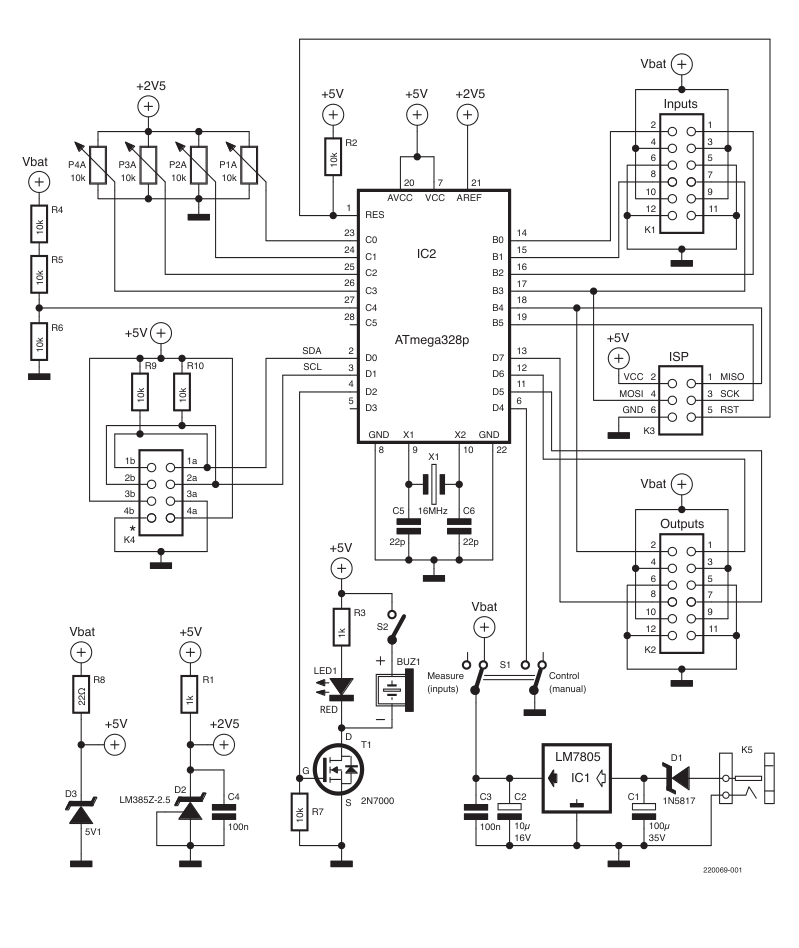
\includegraphics[scale = 0.60]{../img/scrot/Screenshot-2024-05-15-193101.png}
  \caption{Электрическая принципиальная схема устройства}
\end{figure}

На приложенной схеме в центре видно микроконтроллер подключенный к кристаллу с частотой колебаний 16 Мгц, который в свою очередь подключен к конденсаторам C5 и С6. Четыре пина \textit{GPIO} — PB0-PB3 подключены  к разъёму K1. Выводы для серво сигнала — PD5, PD6, PD7 и PB4 подключены к разъёму K2. Два этих раззъёма разведены таким образом, что к ним можно подключлить стандартный для сервопривода кабель ~\cite{Elector521}.

Четыре потенциометра подключеный к аналоговым входам микроконтроллера PC0-PC3. Питание подключается через делитеть напряжения из резисторов R4-R6 к аналоговому входу PC4. Отношение между суммой сопротивлений R4, R5 и сопротивлением R6 должно быть 2 к 1 соотвественно, но их абсолютные значения не критичны. Использование трёх резисторов одного значения облегчает их сортировку для точности ~\cite{Elector521}.

Для того чтобы измерять напряжение источника питания нужен аналогово цифровой преобразователь и 
опорное напряжение не относящиеся к самому напрежению питания.
В микроконтроллере уже есть опорное напряжение в 1,1 Вольт, однако это значение несколько мало. И поэтому используется источник опорного напряжения LM385-2.5 обозначенный как D2, как внешнее опорное напряжение в 2,5 Вольта. Этот элемент более точен, чем простой двухконтактный зенеровский диод ~\cite{Elector521}.

К коннектору K4 подключается \textit{OLED} дислпей по типу SSD1306.
У дисплея должен быть порт \textit{I2C}, но он будет подключаться к порту \textit{I2C} микроконтроллера, но к компонентам PD0 и PD1. Шина \textit{I2C} эмулируется программным обеспечением. Так выходит из-за того, что шина \textit{I2C} на данном микроконтроллере находится на том же пине, что и аналоговый вход PC4, который уже используется для измерения напряжения питания ~\cite{Elector521}.

Резисторы R9 и R10 это подтягивающие резисторы для шины \textit{I2C}.

Ползунковый переключатель S1 типа \textit{DPDT} используется для выбора режима работы тестового стенда. В ручном режиме переключатель соединяет напряжения питания номиналом 5 Вольт и коннекторы сервоприводов. В режиме ввода он предовтращает неправильное включение напряжений ~\cite{Elector521}.

Возможно, что решение в части подключение дисплея к данному тестовому
стенду и не является самым элегантным. Однако сама по себе схема
достаточно проста,состоит из небольшого числа комопонентов, но тем не
менее может работать в нескольких режимах и схемах включения, что выглядит как положительные черты относительно того в каких вариантах использования оказывается устройство.

%%%% Определение параметров
%%%% воздействующих дестабилизирующих факторов и
%%%% протекающих физических процессов

% Приплести сюда ГОСТ на устройство
\subsection{Определение параметров воздействующих дестабилизирующих факторов протекающих физических процессов}


РЭС эксплуатируются в условиях воздействия на них целого ряда
систематических и случайных факторов. Систематические факторы определяют рабочие функции аппаратуры и могут быть учтены в процессе разработки,
а случайные факторы по своему характеру и времени воздействия проявляются случайным образом, в связи с чем учет их влияния в процессе разработки достаточно затруднен ~\cite{Alexeev2013}.

Факторы делятся на объективные, не зависящие от человека, и субъективными, то есть зависящими от действий конструктора или использующего данный тестовый стенд оператора.

По характеру воздействия на РЭС объективные факторы разделяются на климатические, механические и другие.

Параметры климатических факторов принимают значения в соотвестиве с учетом УХЛ 4.2 ГОСТ 15150-69.

Параметры механических факторов же принимают значения, выбранные разработчиком.

Наиболее вероятным механическим фактором для данного устройства будет воздействие вибрации, в следствии работы подключаемых сервоприводов.

Во всей схеме практически не встречаются компоненты с большим тепловыделением. Так например найти коэффициент \textit{TDP} для микроконтроллера не предстовляется возомжным, потому что среди производителй микроконтроллеров, в отличие от производителей микропроцессоров не принято не то что рассчитывать этот коэффициент рассеивания теплоты, а даже закладывать в этот компоенент схемы возможности какого-либо его нагрева.

Однако это ни в коем случае не означает то, что ни один из элементов не будет нагреваться. Напротив при работе любого электронного прибора какая-то часть потребляемой мощности рассеивается как тепло.
Но если рассматривать отношение мощности потребляемой и рассеиваемой как тепло, то можно понять, что самым простым оно будет у резисторов.

По видимому, можно взять информацию о мощности резистора и принять её за мощность рассеиваемую в виде теплоты ~\cite{HeatDissipatedResistors}.

Примерно таким же образом было сделано допущение о схожести в вопросе рассеиваемой мощности между резисторами и потенциометрами.

Исходя из всего вышеописанного был сделан вывод о необходимости проведения частотного анализа и термического анализа.

\newpage

%%% Вторая глава по разделам


\section{Моделирование физических процессов, воздействующих на устройство}
\subsection{Обоснование выбора прикладного программного обеспечения для моделирования физических процессов}

Программ для проведения инженерных расчетов не так уж много. И итак ограниченный выбор пал на три программы: \textit{SOLIDWORKS SIMULATION},
\textit{ANSYS}, \textit{COMSOL Multiphysics}. Дело в том, что все три эти программы, чаще всего и используются для МКЭ расчетов. Хотя, это по большей части относится к \textit{COMSOL Multiphysics} и \textit{ANSYS}, а \textit{SOLIDWORKS} удобен и сам по себе как средство для конвертации, работы и упрощения с трёхмерными параметрическими моделями.
Возможность моделировать в нём можно считать приятным дополненим к его функционалу, которое тем не менее видится как обязательное к использованию в этой работе.

Популярность таких программ как \textit{COMSOL Multiphysics} и \textit{ANSYS} в кругах инженеров позволяет рассчитывать на наличие большого количетства обучающих материалов по ним, в том числе созданных не только самой компанией осуществляющей разработку программы.

Кроме того обе программы сами по себе обладают огромным набором возможностей для проведения симуляции и зачастую имеют некоторый аналог интерфейса трёхмерных параметрических САПР типа \textit{SOLIDWORKS}, который позволяет интерактивно взаимодествовать с геометрией модели, материалом и сеткой модели.

Также особенно хочется отметить доступность и качество документации доступной на официальном сайте \textit{COMSOL}.

Совокупнсот вышеописанных качеств делает эти программы достойным выбором для проведения исследования.

\subsection{Разработка плана моделирования физических процессов}

Под моделированием можно понимать метод исследования, оценок характеристик сложных сечений используемый для принятия решения в различных сферах инженерной деятельности.

Под моделью следует понимать объект заместитель, который в определенных условиях может заменить объект оригинала воспроизводя интересующее исследователя свойство оригинала. Чем более подробное описание модели требуется, тем более длительным и затратным окажется вычислительный
процесс.

Основными целями моделирования является: прогноз (главная цель моделирования), оптимизация и анализ чувствительности.

Следовательно, план моделирование физических процессов выглядит так:
\begin{enumerate}[label={\arabic*.}]
\item Построение нескольких варинтов компоновок исследоваемого тестового стенда.
\item Экспорт получившихся печатных плат в виде трёхмерных моделий пригодных для трёхмерного параметрического моделирования и расчетов методом конечных элементов.
\item Проведение инженерных анализов с использованием различных CAE программ.
\item Сравнение результатов анализиа, полученных из программ.
\item Определние адекватности полученных результатов.  
\end{enumerate}



В случае получения неадекватных результатов моделирование повторяется с первого пункта.

Из этого следует что для более детального анализа необходимо
смоделировать различные варианты компоновки тестового стенда, а также
смоделировать и проанализировать, для каждого варианта исполнения,
результаты физических процессов. Моделирование будет проводится до тех
пор, пока не будут получены адекватные результаты.


\subsection{Методика построения трехмерной модели исследуемого устройства}

Создание модели печатной платы было начато в САПР \textit{Altium Designer}.
В нём была создана библиотека УГО принципиальная схема устройства.
Затем, по логике создания моделей в САПР печатных плат подобных \textit{Altium Designer} должны были быть созданы библиотеки посадочных мест, соедиение их с УГО размещенных на принципиальной схеме.
После чего надо было бы разнести посадочные места на печатной плате и произвести трассировку.

Однако я поступил не так.
Из-за своего изначального предпочтения к использовонию программ с открытым исходным кодом было принято решение использовать САПР печатных плат \textit{KiCAD}.

В тот момент процедура создания печатных плат в \textit{KiCAD}, казалась проще, чем в \textit{Alitum Designer}. Всё дело в том, что у \textit{KiCAD} существует своя библиотека посадочных мест с трёхмерными моделями соотвествующих компонентов в формате \textit{STEP} и \textit{WRL}. Также на \textit{Github} была найдена готовая библиотека УГО соотвествующая ГОСТ.
В \textit{KiCAD} нет предустановленного встроенного автотрассировщика и потому разводка платы производилась вручную,
несмотря на то что можно было бы установить автотрассировщик \textit{freerouting}.

На этом этапе казалось, что выбор \textit{KiCAD} в качестве САПР печатных плат всё только упрощает, поскольку теперь было достаточно:
\begin{enumerate}[label={\arabic*.}]
\item Создать схему электрическую принципиальную, используя готовую библиотеку УГО.
\item На схеме установить соотвествие между УГО и посадочными местами, у которых есть свои трёхмерные модели.
\item Импортировать получившиеся связи непосредственно в документ, в котором осуществляется разводка печатной платы.
\item Рапределить компоненты в группы и провести дорожки наиболее эффективных способом.
\end{enumerate}

Это и было сделано. На тот момент подозрений о том, что это приведёт к каким-либо проблемам не было.

\begin{figure}[H]
  \centering
  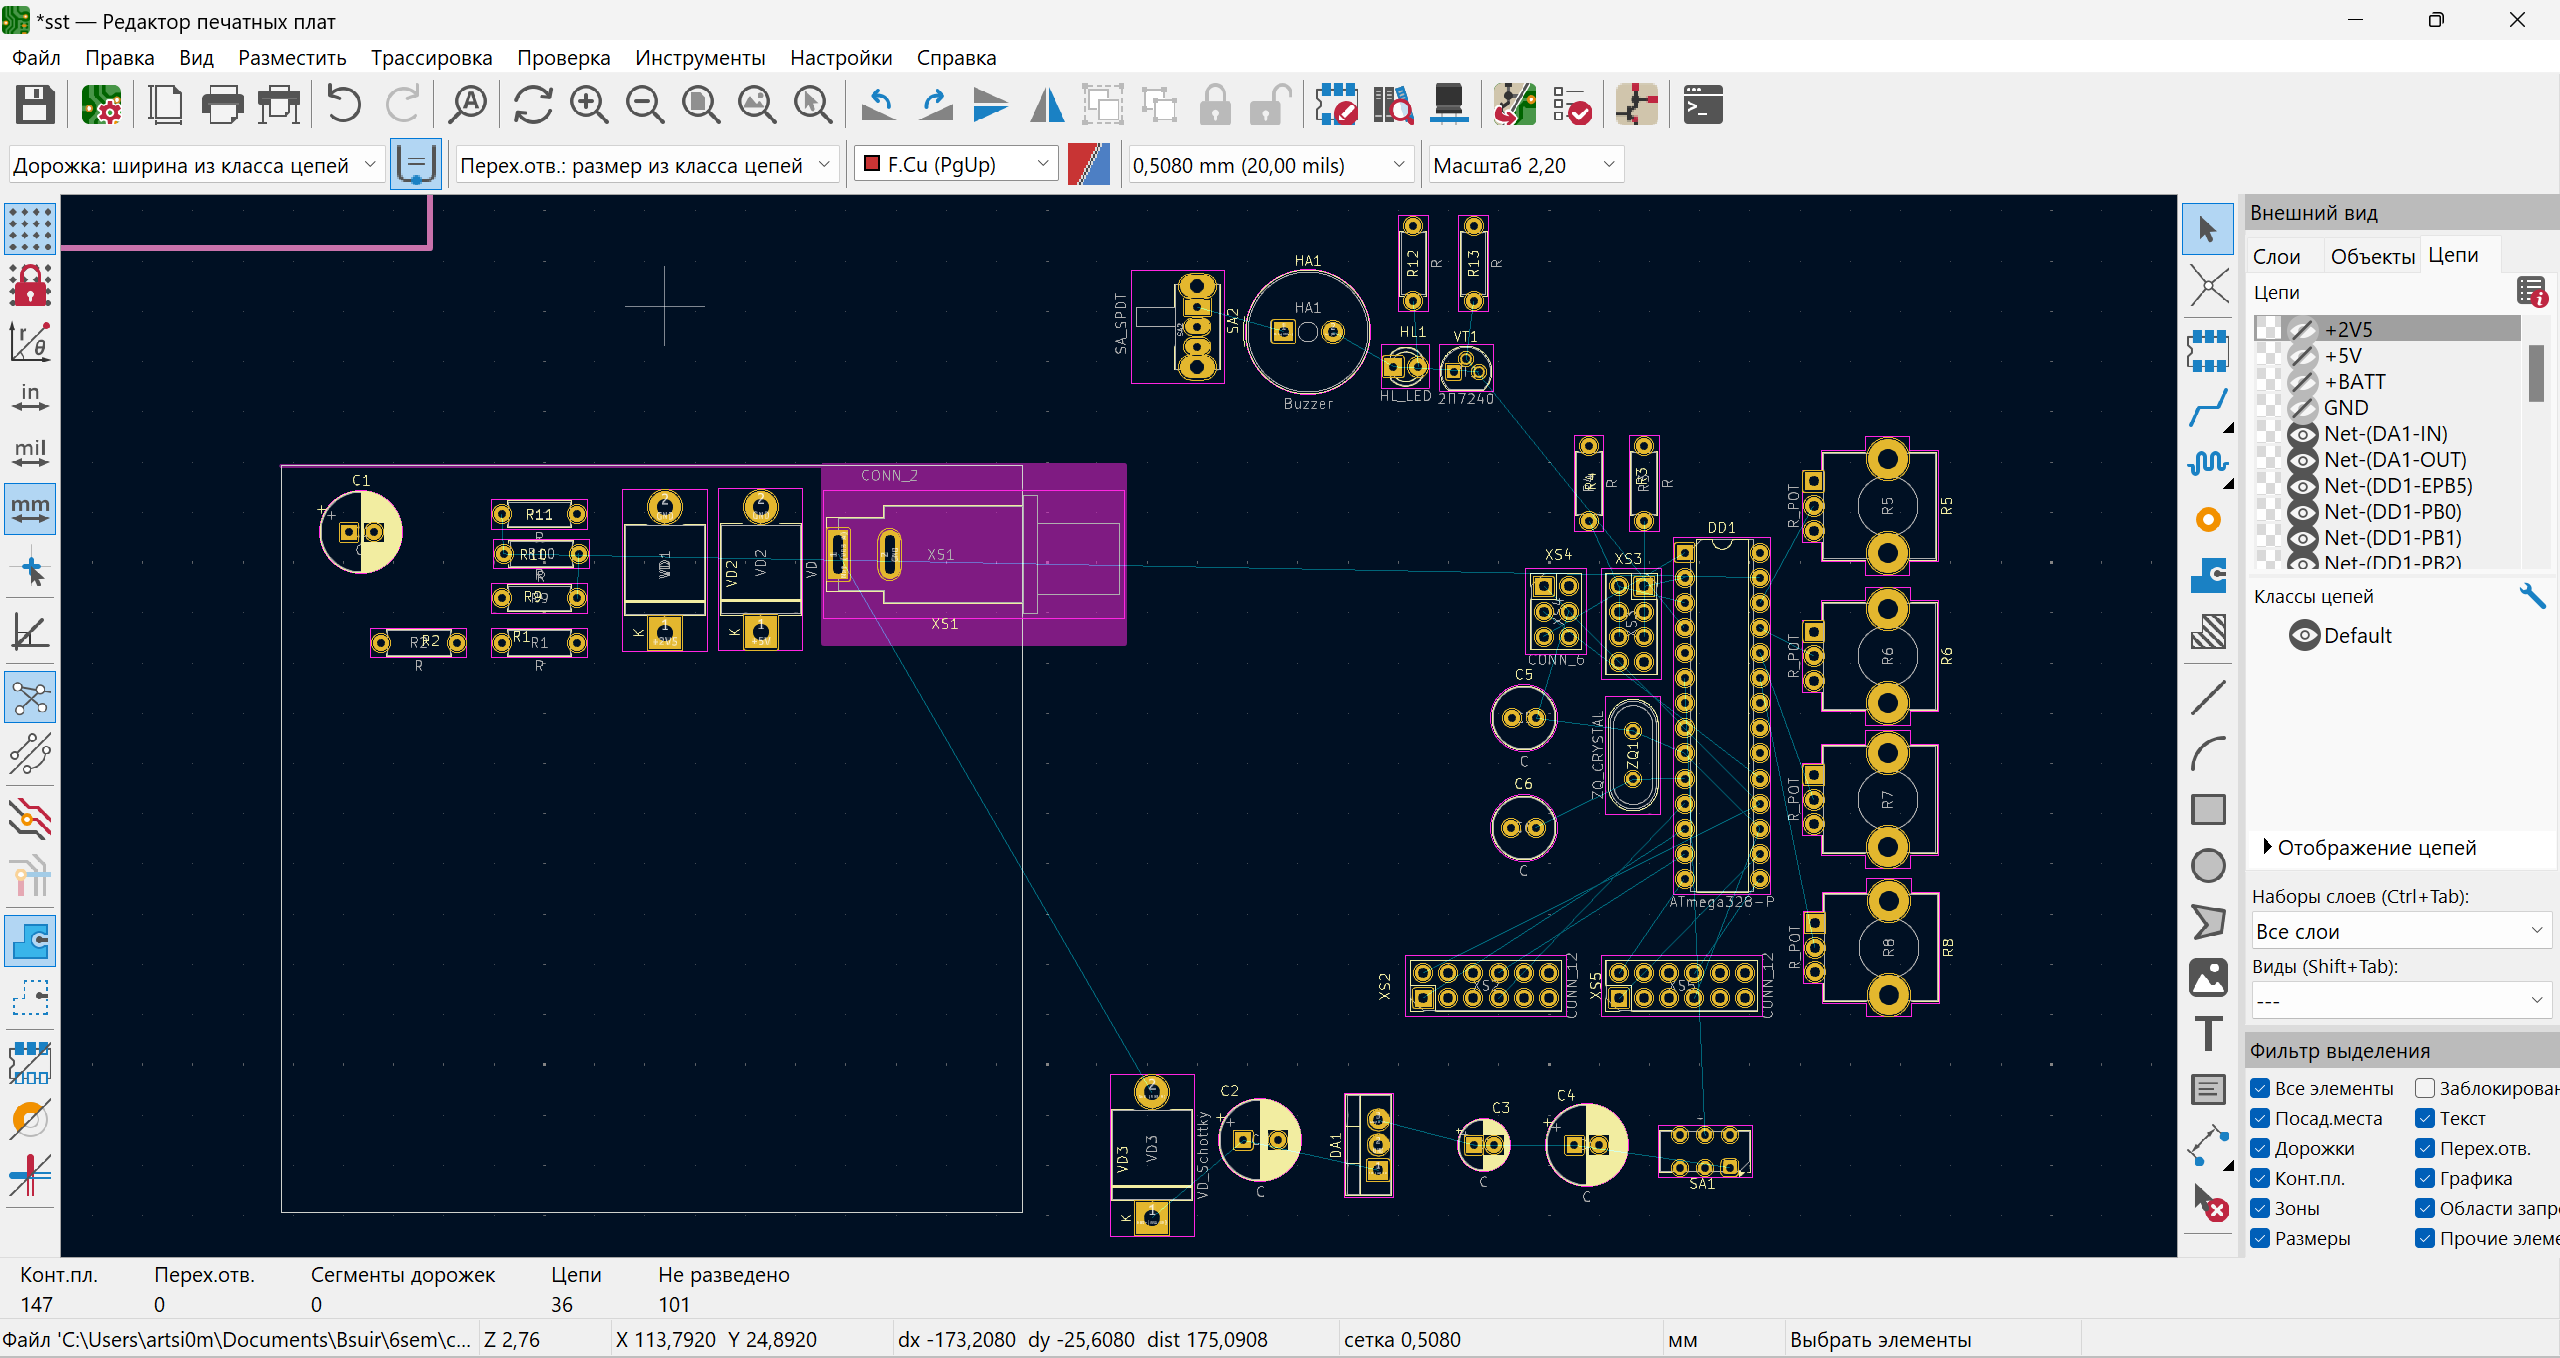
\includegraphics[scale = 0.20]{../img/scrot/Screenshot-2024-05-02-173914.png}
 \caption{Скриншот окна САПР \textit{KiCAD} в котором скрыты цепи относящиеся к питанию и компоненты распределены по группам.}
\end{figure}

Была произведена разводка первой печатной платы:
сначала скрыты цепи связанные с питанием, затем компоненты были объеденены в группы, после чего расставлены по контуру печатной платы и соедены дорожками.

Чтобы заново не производить разводку, а если быть предельно точным,
соединение компонентов было сделать две последующие компоновки печатной платы следующим способом:


В случае второй компоновки просто заменить расположение некоторых посадочных мест, таким образом, чтобы они оказались на другой стороне печатной платы, но подали в нужные отверстия печатной платы. В основном это относилось к резисторам, которые в последствии были использованы, как элементы выделяющие тепло в термическом анализе.


В случае третьей платы были заменены некоторые посадочные места, на минитюаризированные аналоги, в описании которых при этом значился тот же самый шаг (\textit{pitch}) между отверстиями.

\begin{figure}[H]
  \centering
  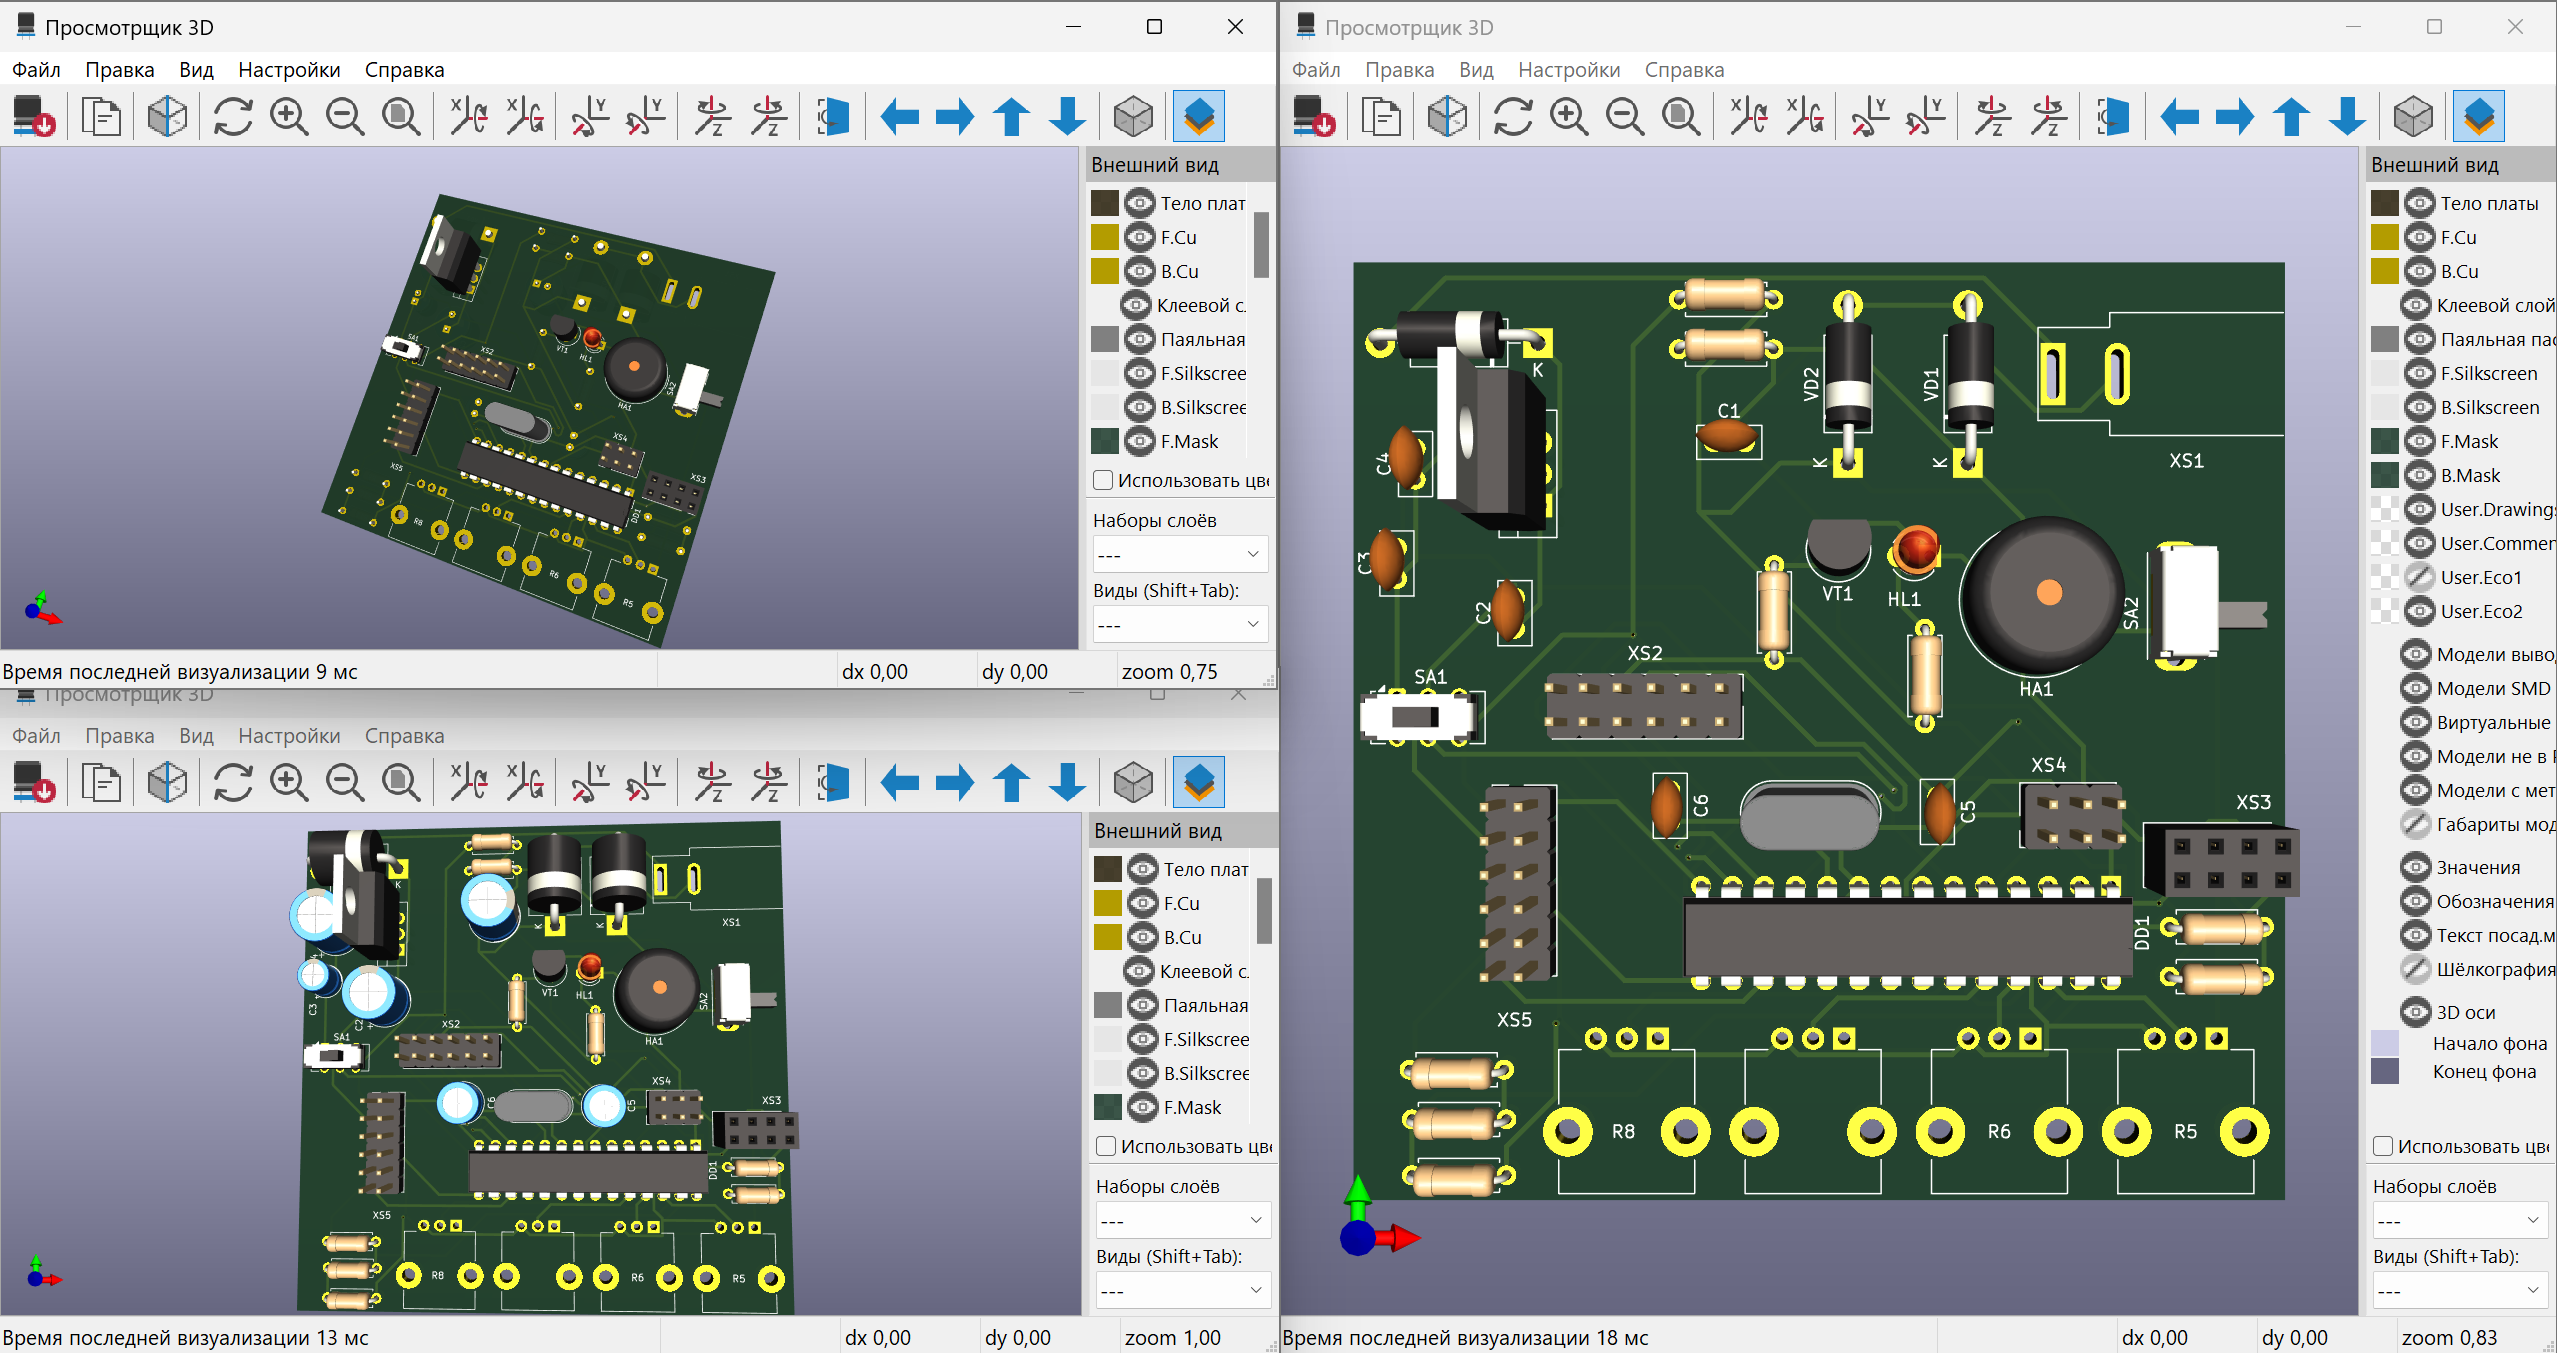
\includegraphics[scale = 0.20]{../img/scrot/Screenshot-2024-05-07-112847.png}
 \caption{Скриншот окон просмотрщика трёхмерных моделей САПР \textit{KiCAD}}
\end{figure}


Полученные варианты печатной платы необходимо экспортировать в \textit{SOLIDWORKS} для проведения дальньшей симуляции. И вот здесь возникли проблемы с получившийся моделью.

\begin{figure}[H]
  \centering
  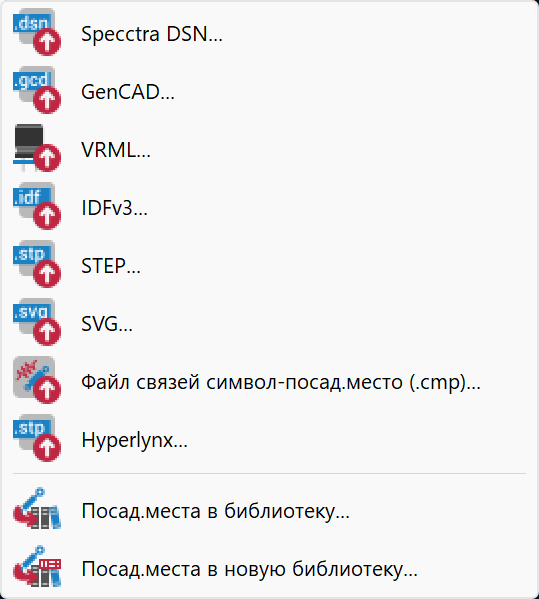
\includegraphics[scale = 0.4]{../img/scrot/Screenshot-2024-05-06-191242.png}
  \caption{Скриншот меню экспорта печатной платы в САПР \textit{KiCAD} }
\end{figure}

В первую очередь была осуществлена попытка экспортировать печатную плату из \textit{KiCAD} в формате \textit{STEP}. Конечно же модель успешно экспортировалась. Проблема была в другом: полученная модель была излишне подробна. Расчет такой модели в \textit{SOLIDWORKS Simulation} мог занимать по пять минут для частотного анализа, но, что более критично, часто приводил к зависанию или падению \textit{SOLIDWORKS}.

Для того, чтобы решить эту проблему было предпринята попытка экспортировать в формате \textit{IDFv3}. Это решение было принято из-за того, что подразумевалось,
что при импорте полученного \textit{IDF} файла в \textit{SOLIDWORKS} будет автоматически использовано дополнение \textit{Circuit WORKS}, которое в случае импорта из \textit{Аltium Designer} упрощало модель таким образом, что вместо точных трехмерных моделей компонентов получались схожие, но значительно упрощенные трёхмерные геометрические фигуры.


\begin{figure}[H]
  \centering
  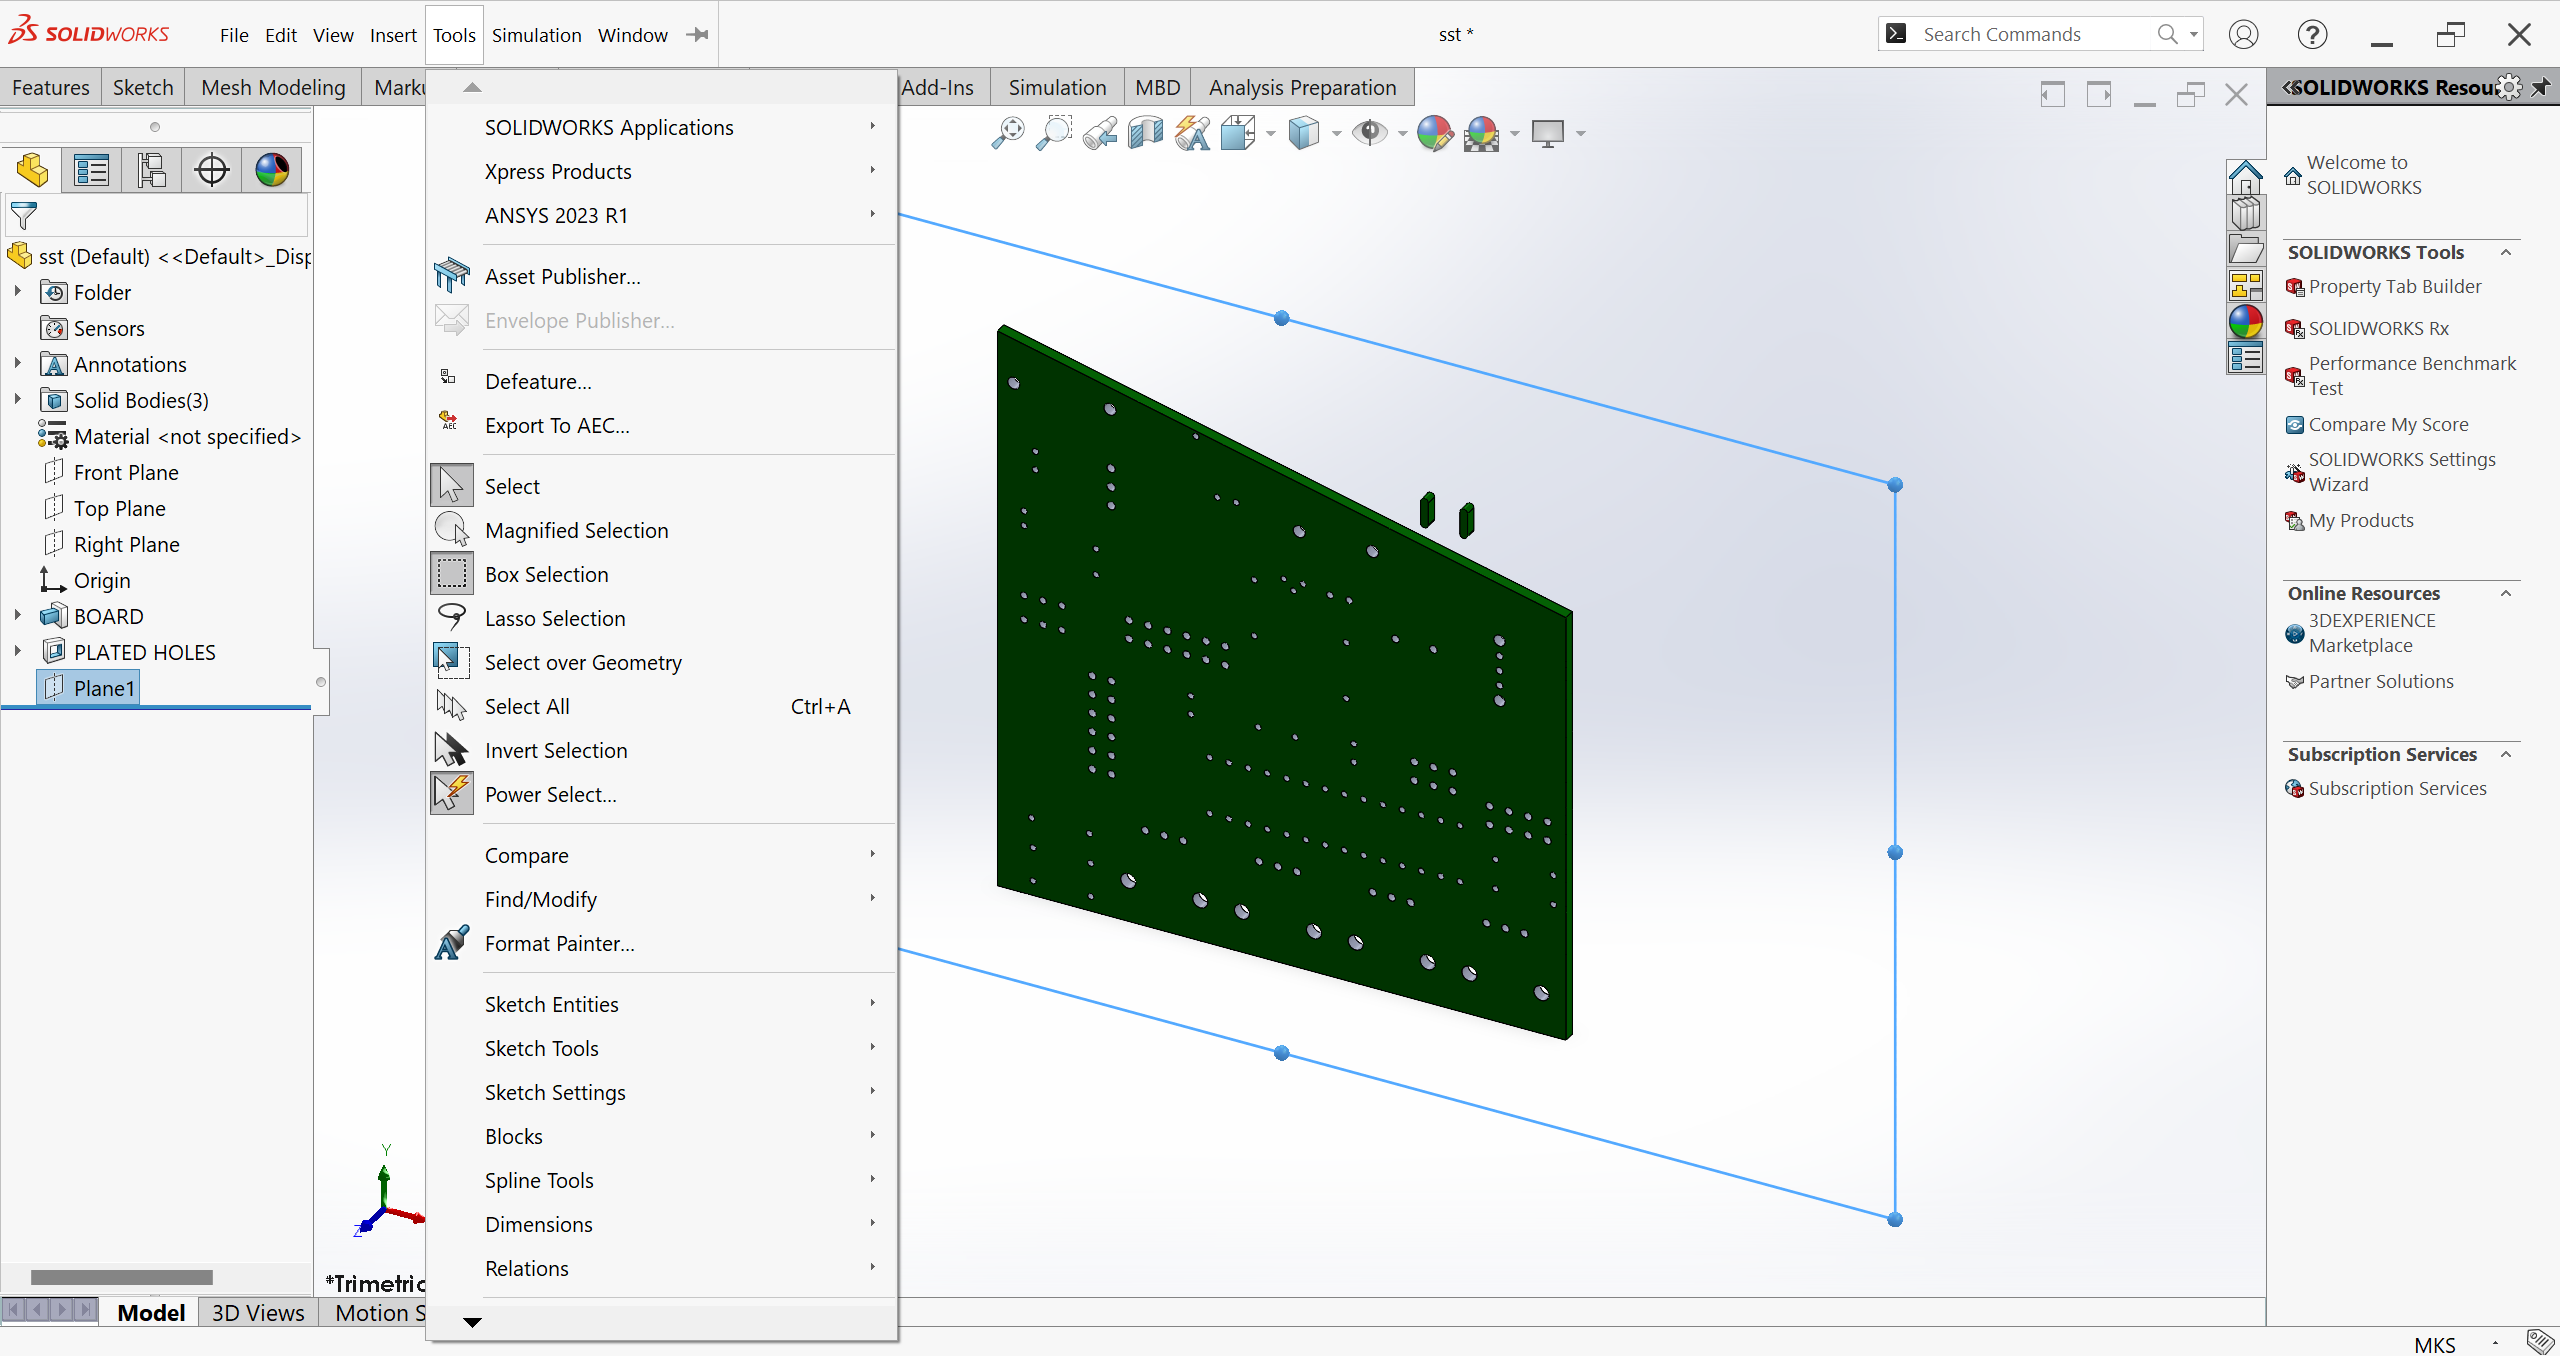
\includegraphics[scale=0.2]{../img/scrot/Screenshot-2024-05-06-175849.png}
  \caption{Скриншот импортированного IDF печатной платы в САПР \textit{SOLIDWORKS}}
\end{figure}

Однако и эта попытка кончилась провалом. Импортированная плата не имела вообще никаких компонентов и была упрощена черезмерно.

Было понятно, что нужно будет переделывать в \textit{Altium Designer} какую-то часть проекта, чтобы получить полноценную трёхмерную модель печатной платы.

Однако совсем не хотелось терять проделанную работу, поэтому было установлено расширение для \textit{Altium Designer} под названием \textit{KiCAD Importer}, которое предоставляло мастер импорта проектов из \textit{KiCAD}.

\begin{figure}[H]
  \centering
  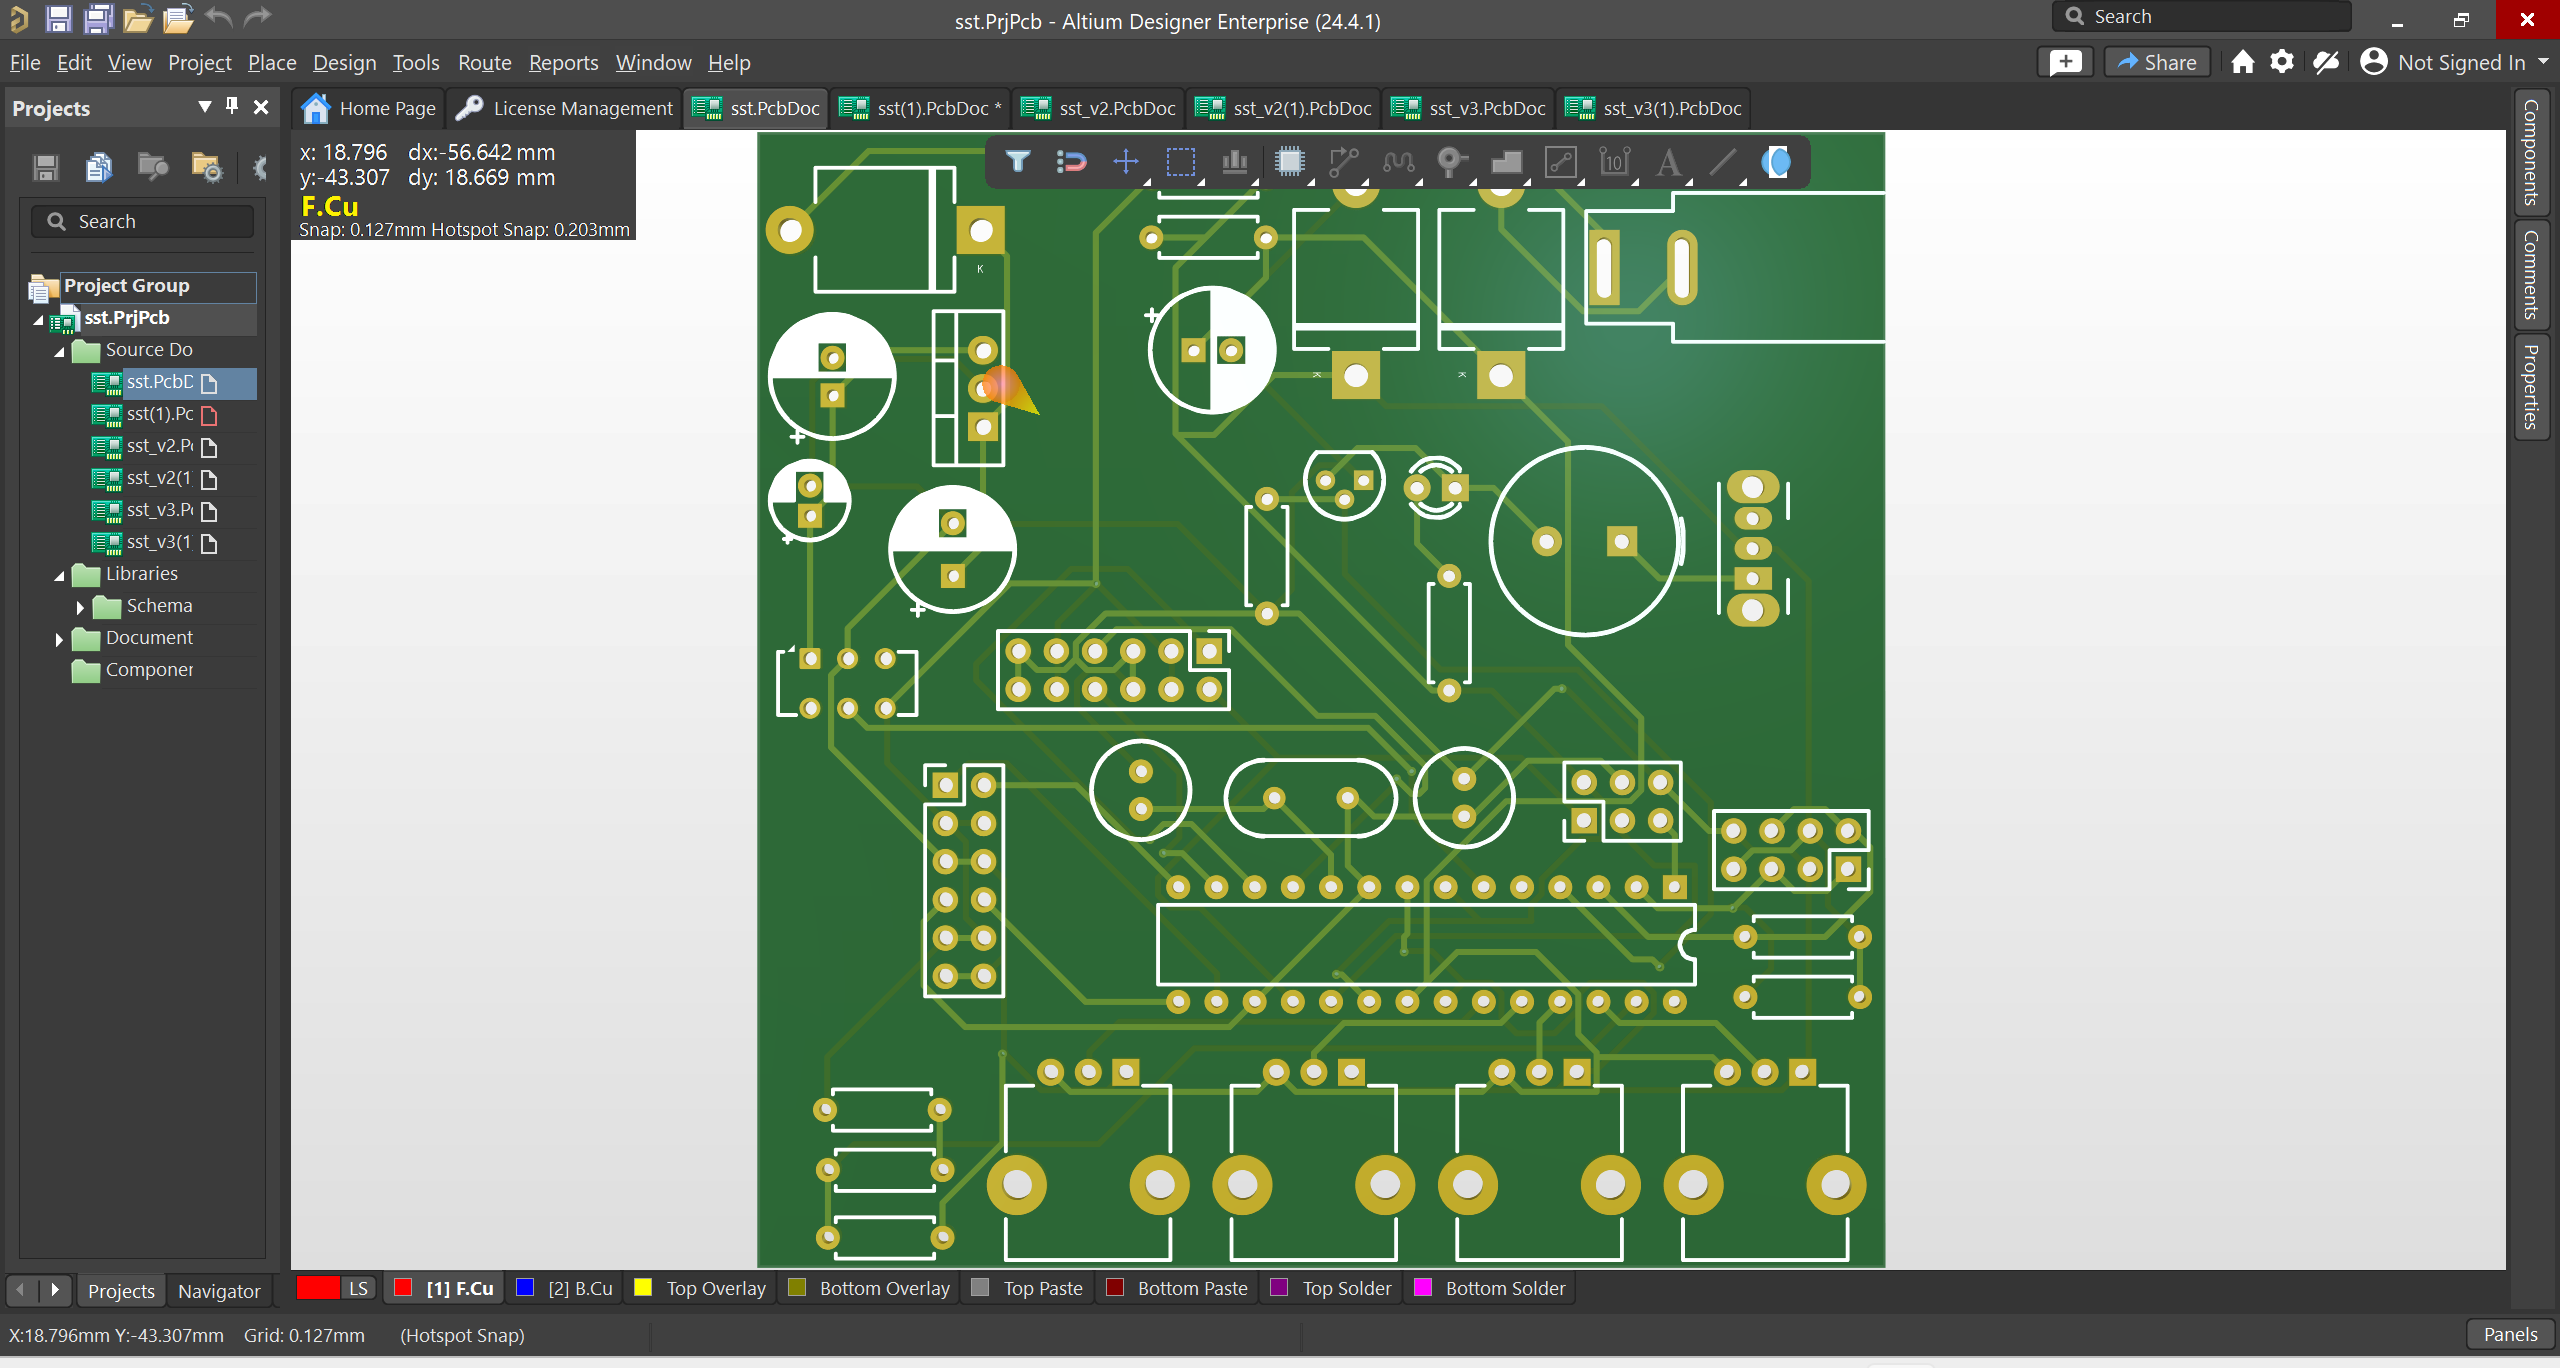
\includegraphics[scale=0.2]{../img/scrot/Screenshot-2024-05-08-110214.png}
  \caption{Скриншот трёхмерной модели имопрированной из \textit{KiCAD} печатной платы в \textit{Altium Designer}}

\end{figure}

В результате импорта в проекте \textit{Altium} появились соотвественно три документа печатных плат.

После этого модели были экспортированы из \textit{Altium} в формате \textit{IDF}. Затем был осуществлен импорт этих моделей в \textit{SOLIDWORKS}. В отличие от моделей получившихся при предыдущей попытке экспорта теперь была сохранена геометрия платы и остались контуры (\textit{Sketch}) от элементов расположенных на ней. В последствии инструментом \textit{Extrude} на вкладке \textit{Analysis Prepartion} было осуществлено выдавливание фигур, схожих по объёму с трехмерным моделями печатных плат.

\begin{figure}[H]
  \centering
  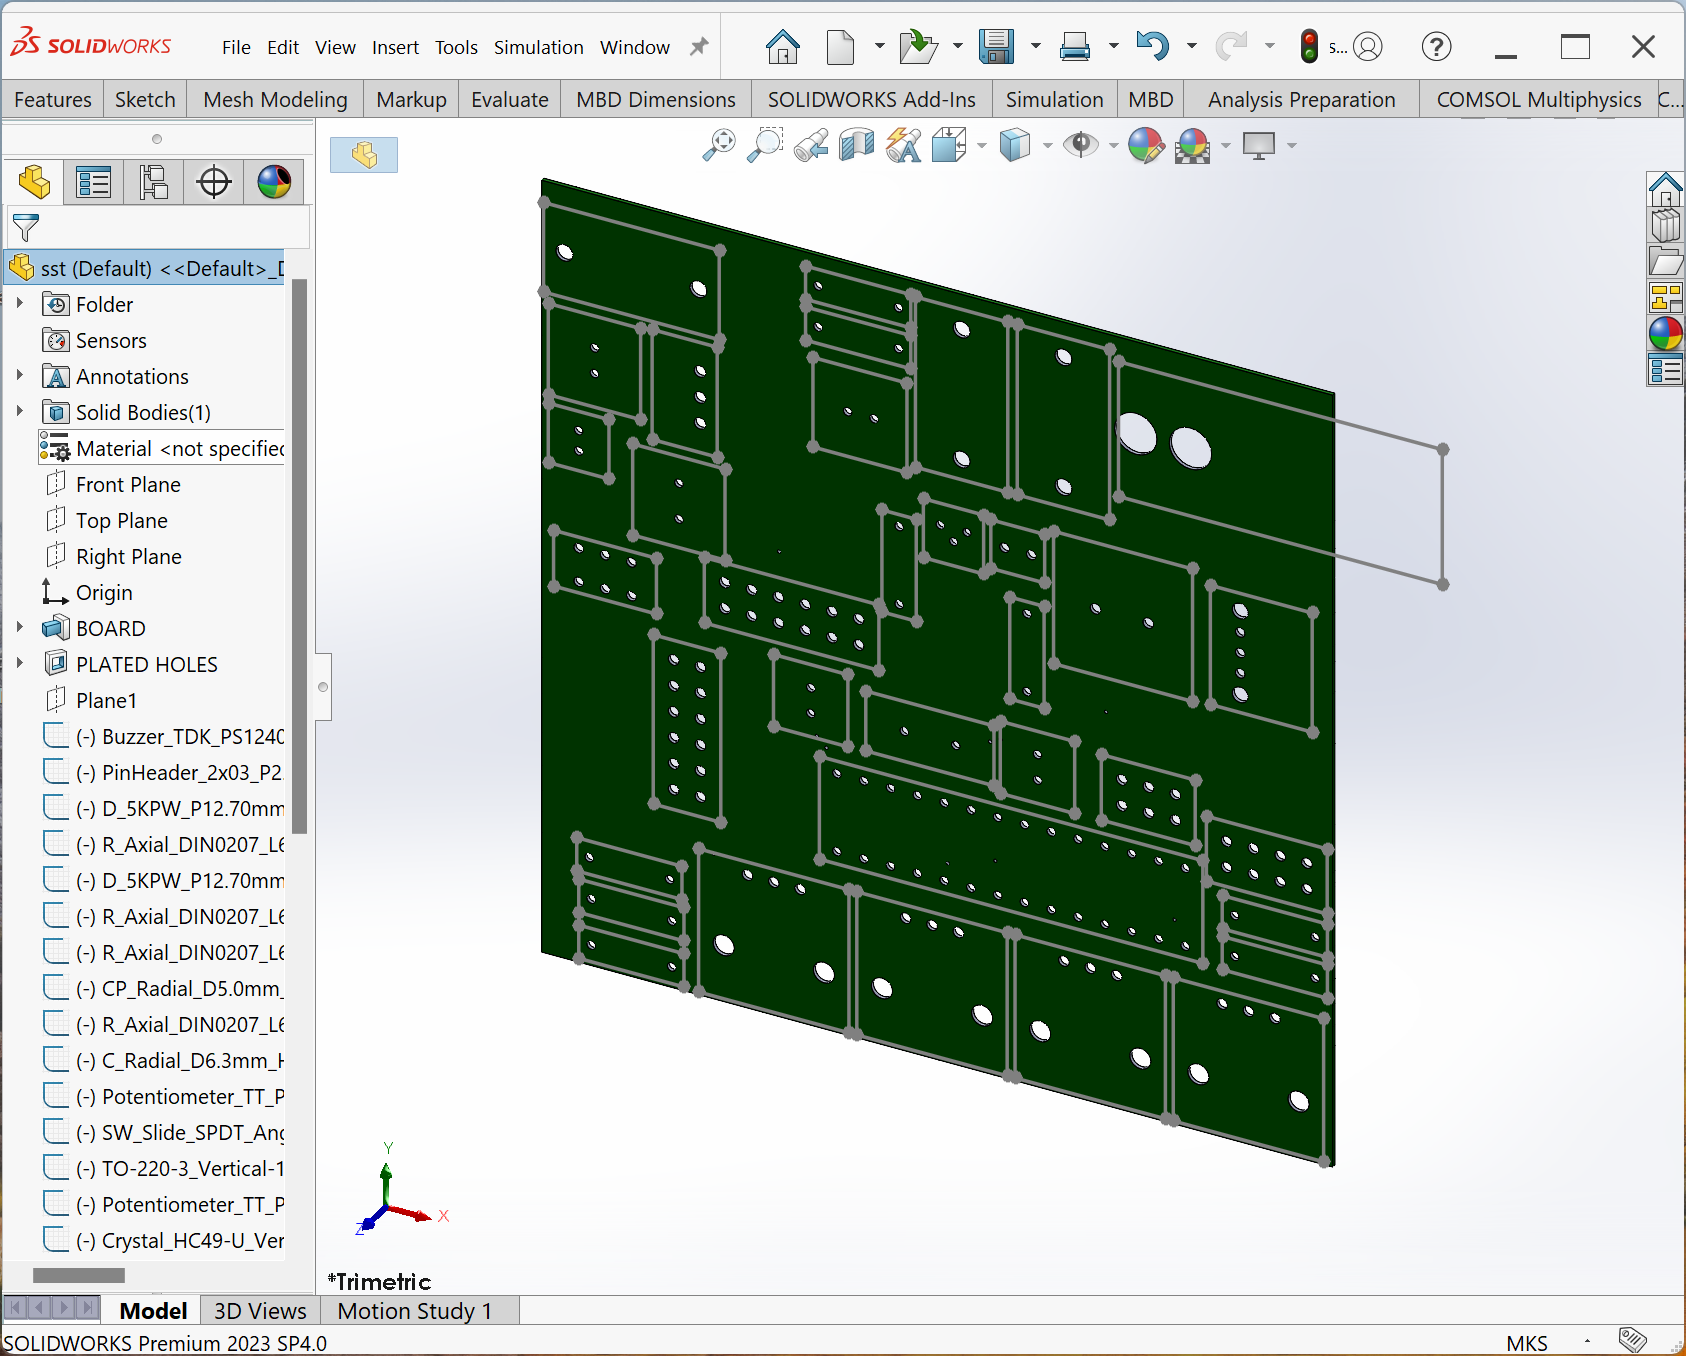
\includegraphics[scale=0.3]{../img/scrot/Screenshot-2024-05-08-132748.png}
  \caption{Скриншот только импортированной в \textit{SOLIDWORKS} печатной платы в формате IDF из \textit{Altium Designer}. Видны контуры посадочных мест.}

\end{figure}


Изначально зная о том, сколько работы будет потрачено, на всего лишь, экспорт трёхмерной модели печатной платы я бы не стал использовать для этого САПР \textit{KiCAD} даже несмотря на возможное удобство в непоредственно проектировании.

Из этого можно сделать вывод, что при выполнение подобных проектов, при выбьоре определенного САПР стоит руководствоваться совместимостью его с другими программами.
Или хотя бы заренее проверять на каком-то миниатюрном проекте-приемере возможность перенесения модели из одной программы в другую.

Что же касается непосредственно проектирвония, то, возможно, было опрометчиво отказываться от использования монтажных отверстий в плате.



\subsection{Моделирование механических процессов, проетекающих в электронном модуле и устройстве в целом}

Результаты частотного анализа в \textit{SOLIDWORKS Simulation} первого варианта компоновки ПП представлены на рисунке 8.

\begin{figure}[H]
  \centering
  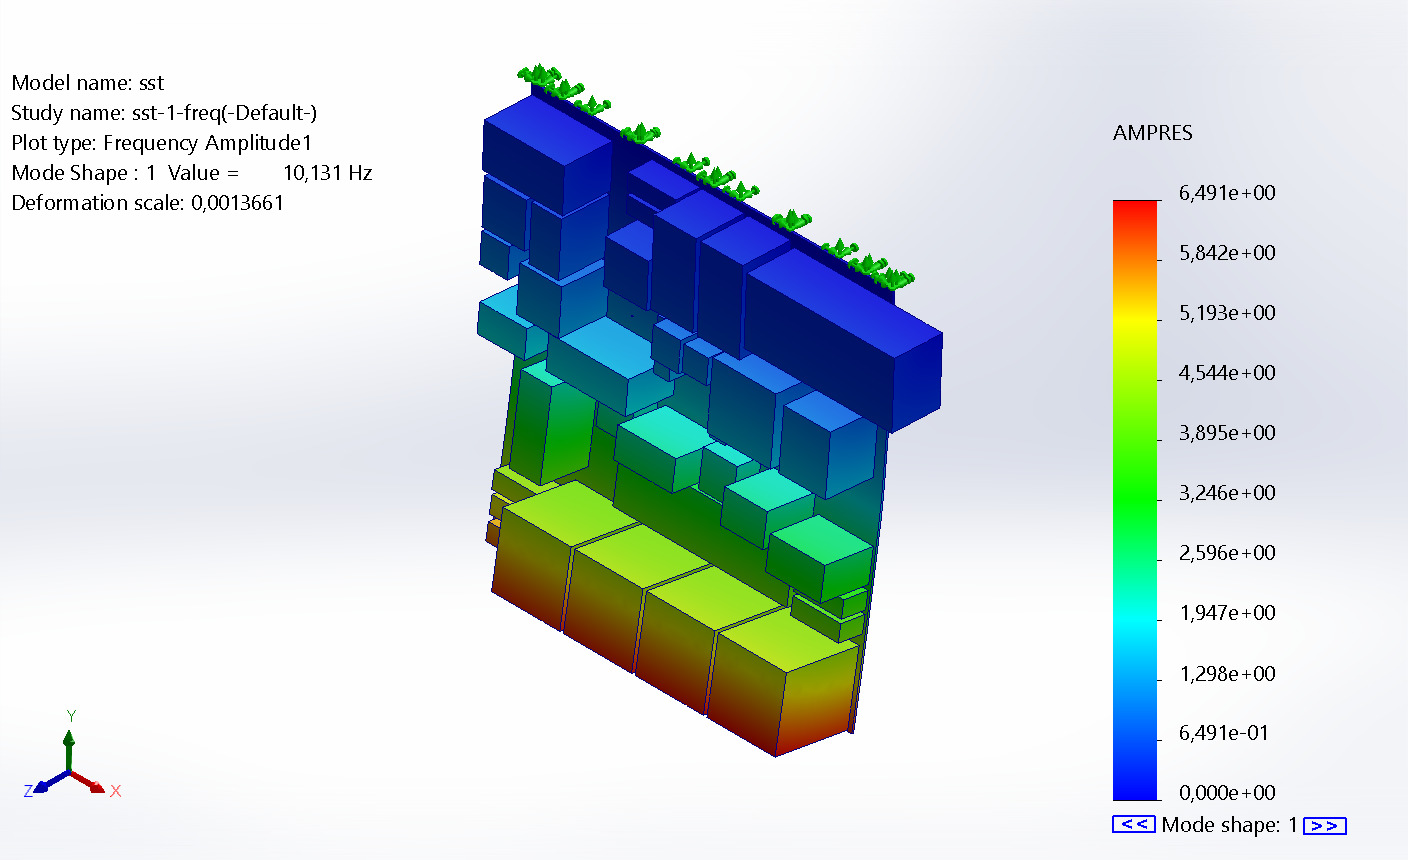
\includegraphics[scale=0.3]{../img/sst-1/freq/top_view/sst-sst-1-freq-Amplitude-Amplitude1.jpg}
  \caption{Результаты частотного анализа в \textit{SOLIDWORKS SIMULATION} первого варианта компоновки ПП.}
\end{figure}


На рисунке 9 представлены результаты частотного анализа в \textit{SOLIDWORKS Simulation} второго варианта компоновки печатной платы.

\begin{figure}[H]
  \centering
  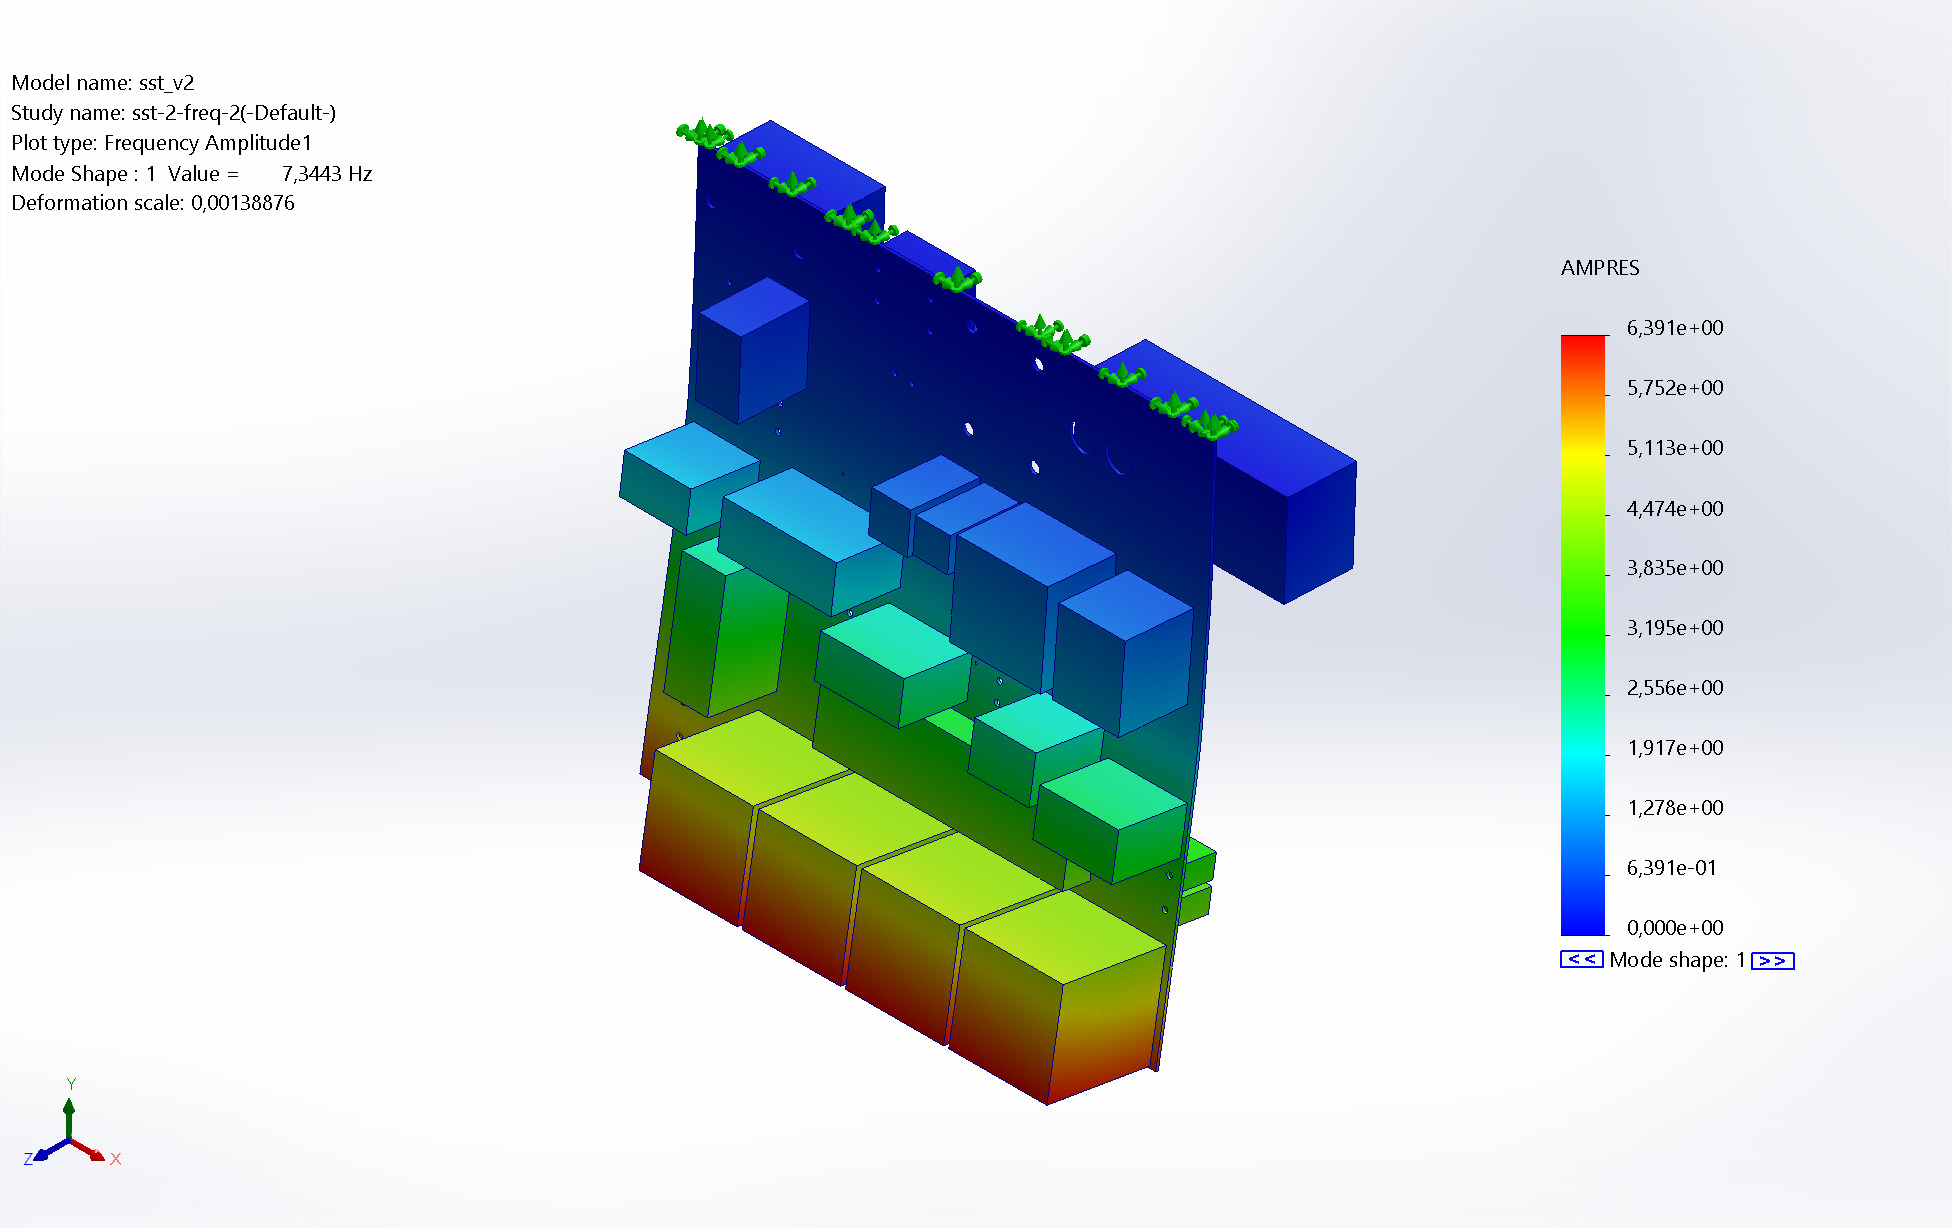
\includegraphics[scale = 0.3]{../img/sst-2/freq/sst_v2-sst-2-freq-2-Amplitude-Amplitude1.jpg}
  \caption{Результаты частотного анализа в \textit{SOLIDWORKS SIMULATION} второго варианта компоновки ПП.}

\end{figure}

На рисунке 10 представлены результаты частотного анализа в
\textit{SOLIDWORKS Simulation} третьего варианта компоновки печатной платы.


\begin{figure}[H]
  \centering
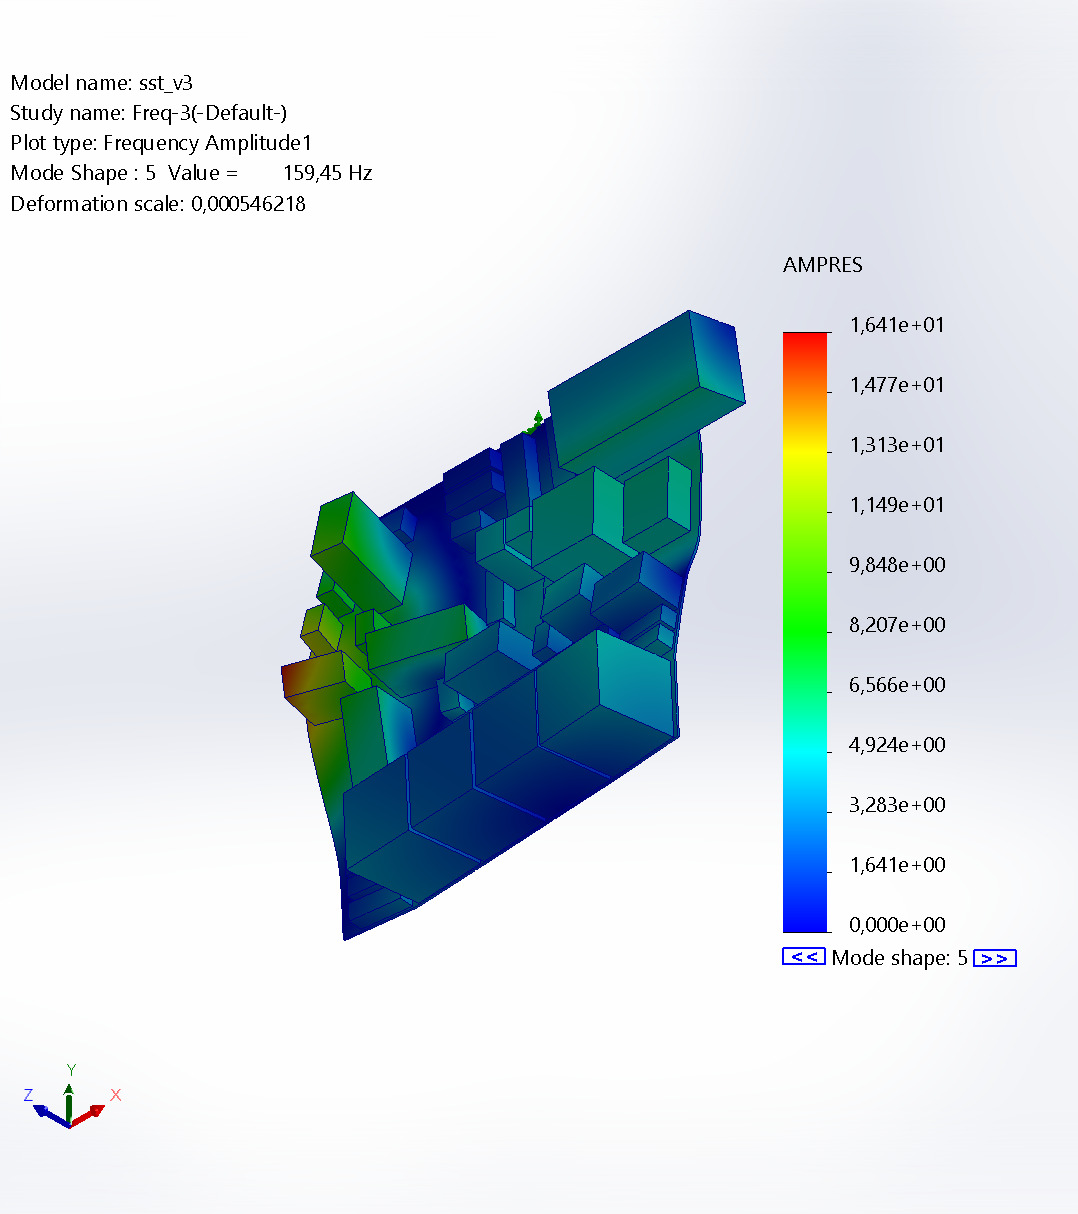
\includegraphics[scale=0.3]{../img/sst-3/freq/sst_v3-Freq-3-Amplitude-Amplitude1.jpg}
\caption{Результаты частотного анализа в \textit{SOLIDWORKS Simulation} третьего варианта компоновки ПП.}
\end{figure}

На рисунке 11 представлены результаты частотного анализа в
\textit{COMSOL Multiphysics} первого варианта компоновки печатной платы.

\begin{figure}[H]
  \centering
  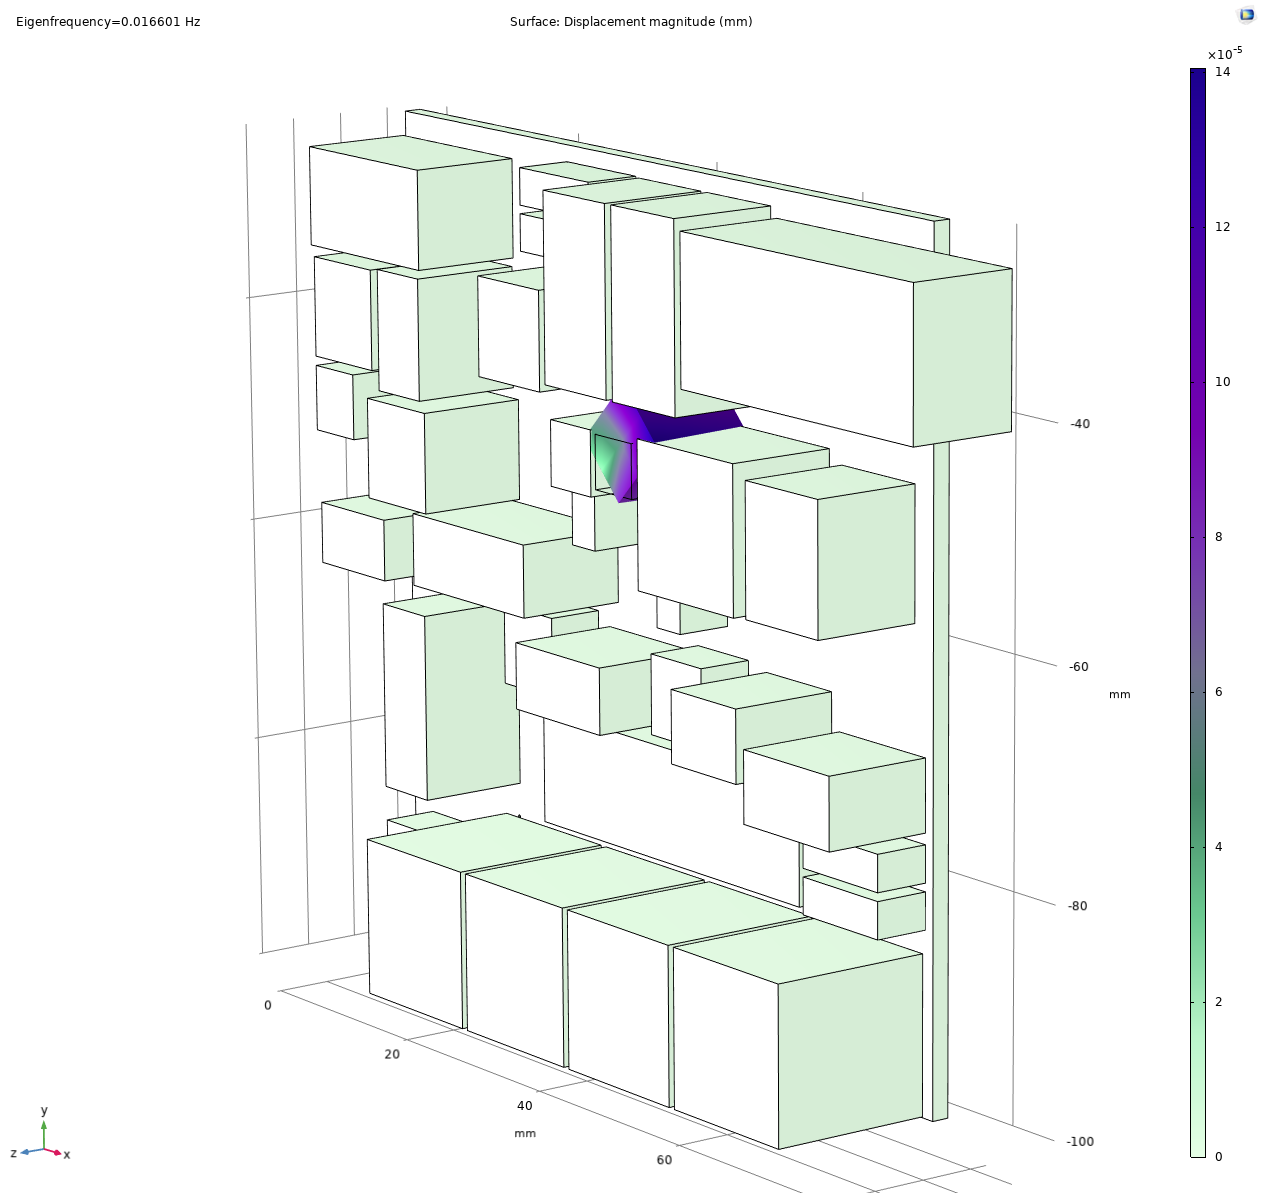
\includegraphics[scale=0.3]{../img/sst-1/freq/comsol.png}
  \caption{Результаты частотного анализа в \textit{COMSOL Multiphysics} первого варианта компоновки}
\end{figure}

На рисунке 12 представлены результаты частотного анализа в \textit{COMSOL Multiphysics} второго вараинта компоновки печатной платы.

\begin{figure}[H]
  \centering
  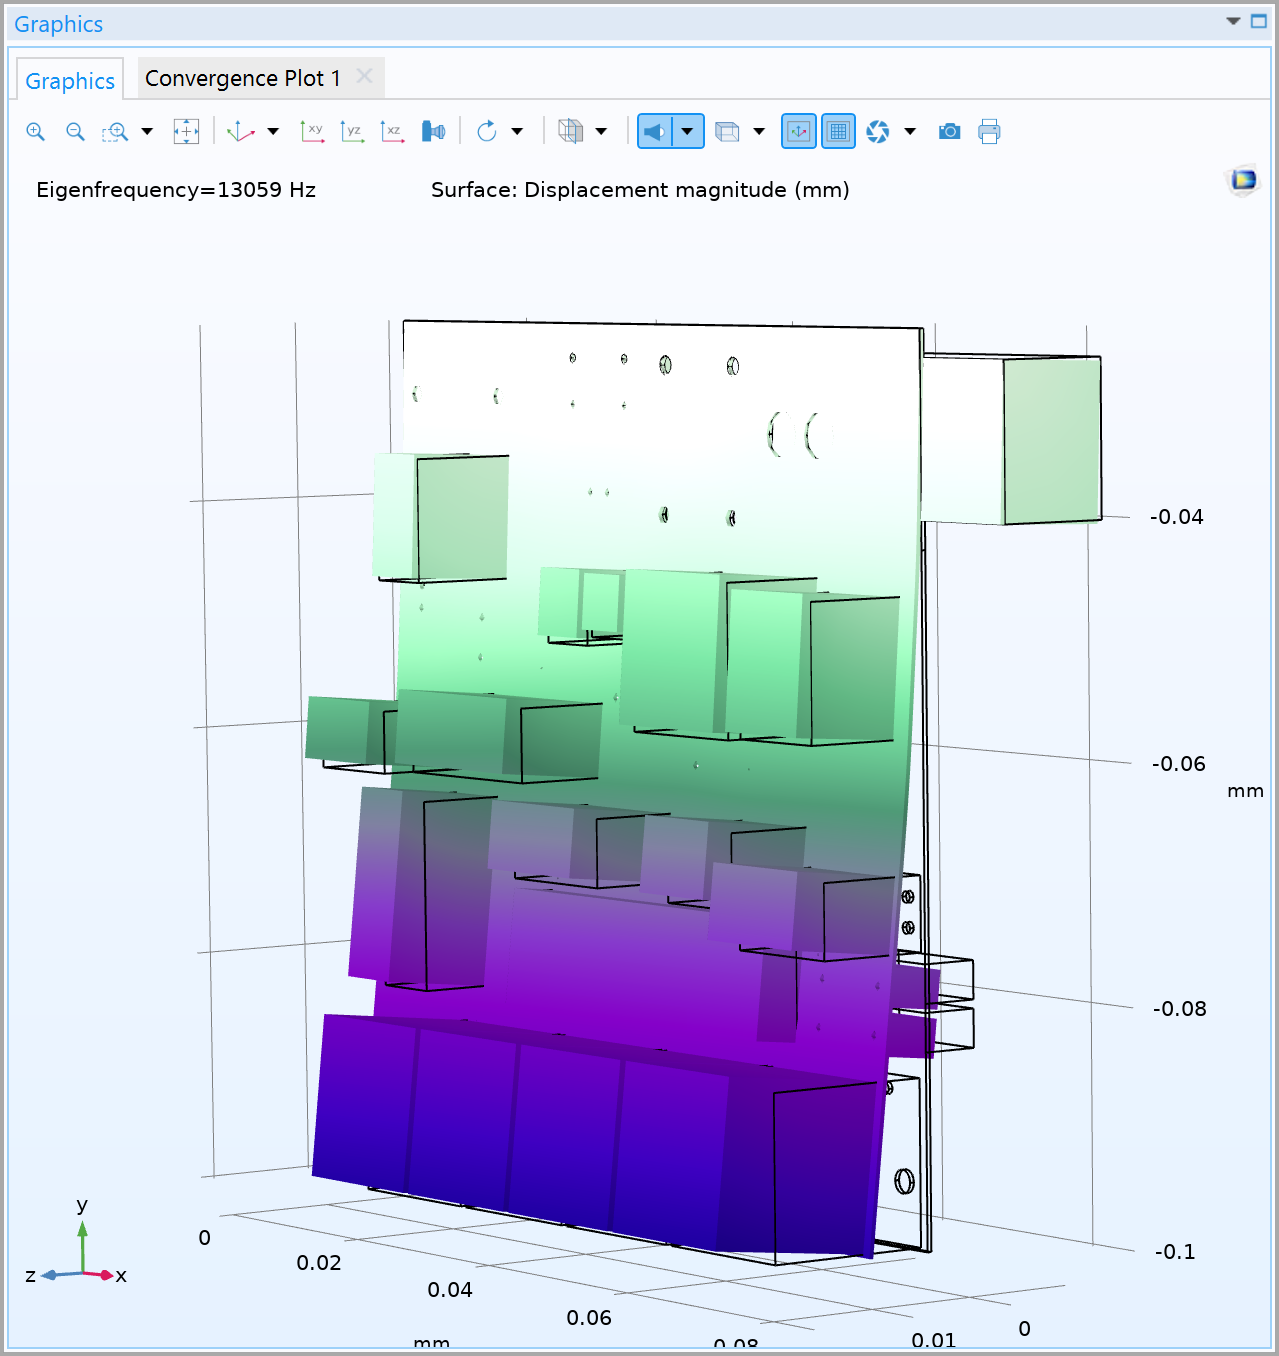
\includegraphics[scale=0.3]{../img/scrot/Screenshot-2024-05-16-014808.png}
  \caption{Результаты частотного анализа в \textit{COMSOL Multiphysics}
    второго варианта компоновки}
\end{figure}

На рисунке 13 представлены результаты частотного анализа в \textit{COMSOL Multiphysics} третьего варианта компоновки печатной платы.

\begin{figure}[H]
  \centering
  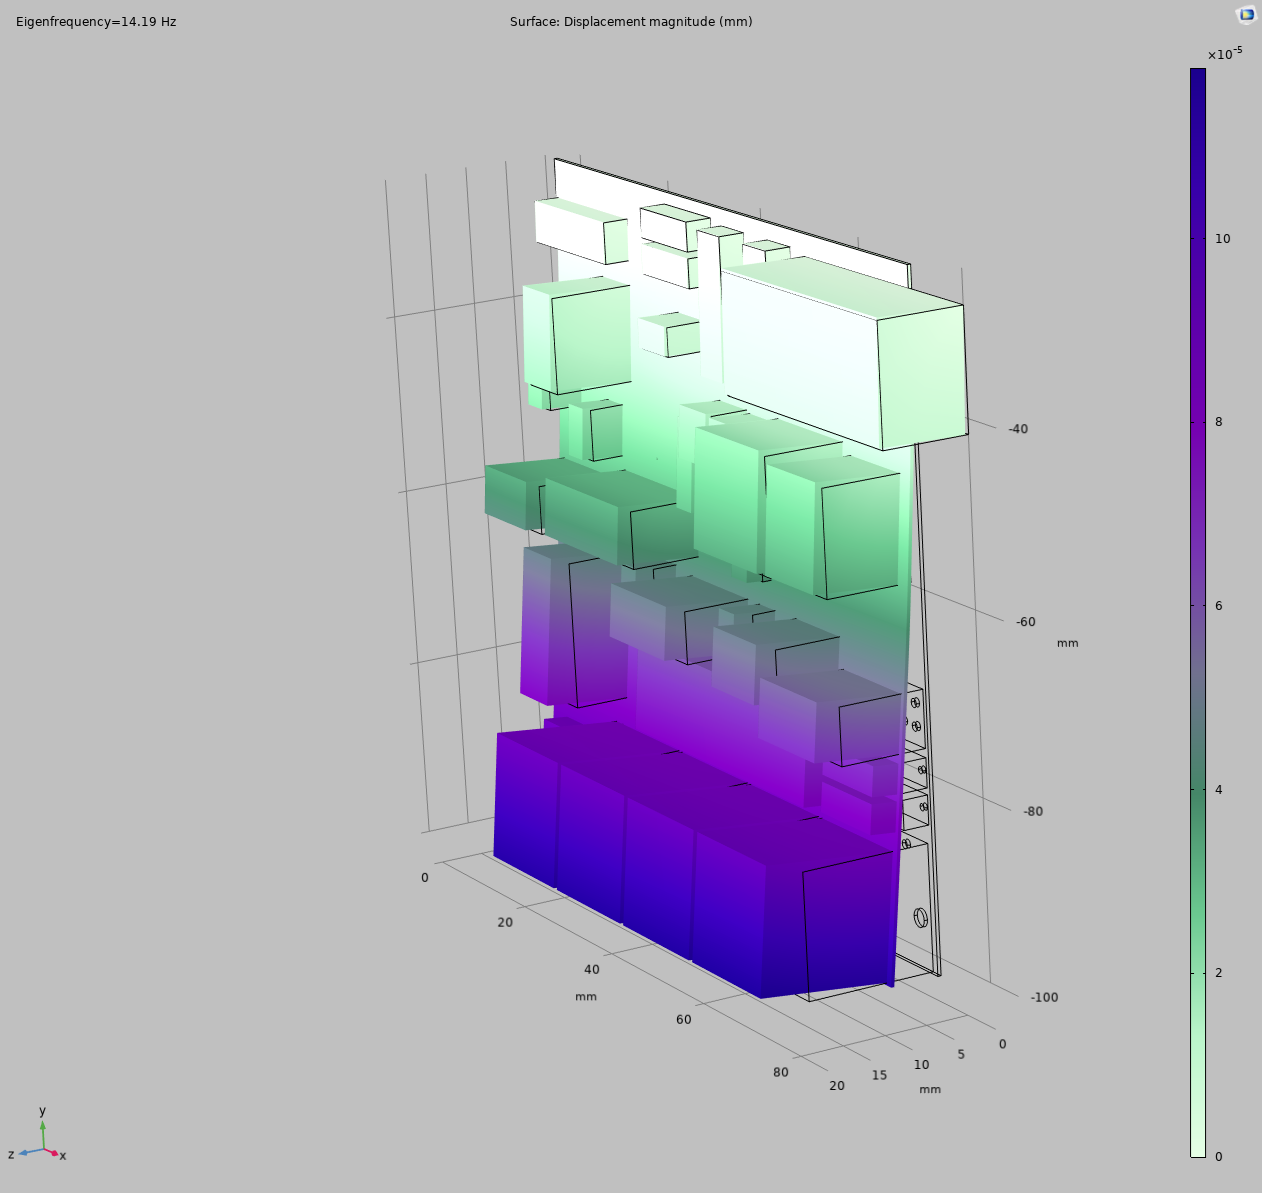
\includegraphics[scale=0.3]{../img/sst-3/freq/comsol.png}
  \caption{Результаты частотного анализа в \textit{COMSOL Multiphysics}
    третьего варианта компоновки}
\end{figure}


\subsection{Моделирование тепловых процессов, протекающих в электронном модуле и устройстве в целом}

Результаты теплового анализа для первого варианта компоновки ПП
в \textit{SOLIDWORKS Simulation} представлены на рисунке 14.

\begin{figure}[h]
  \centering
  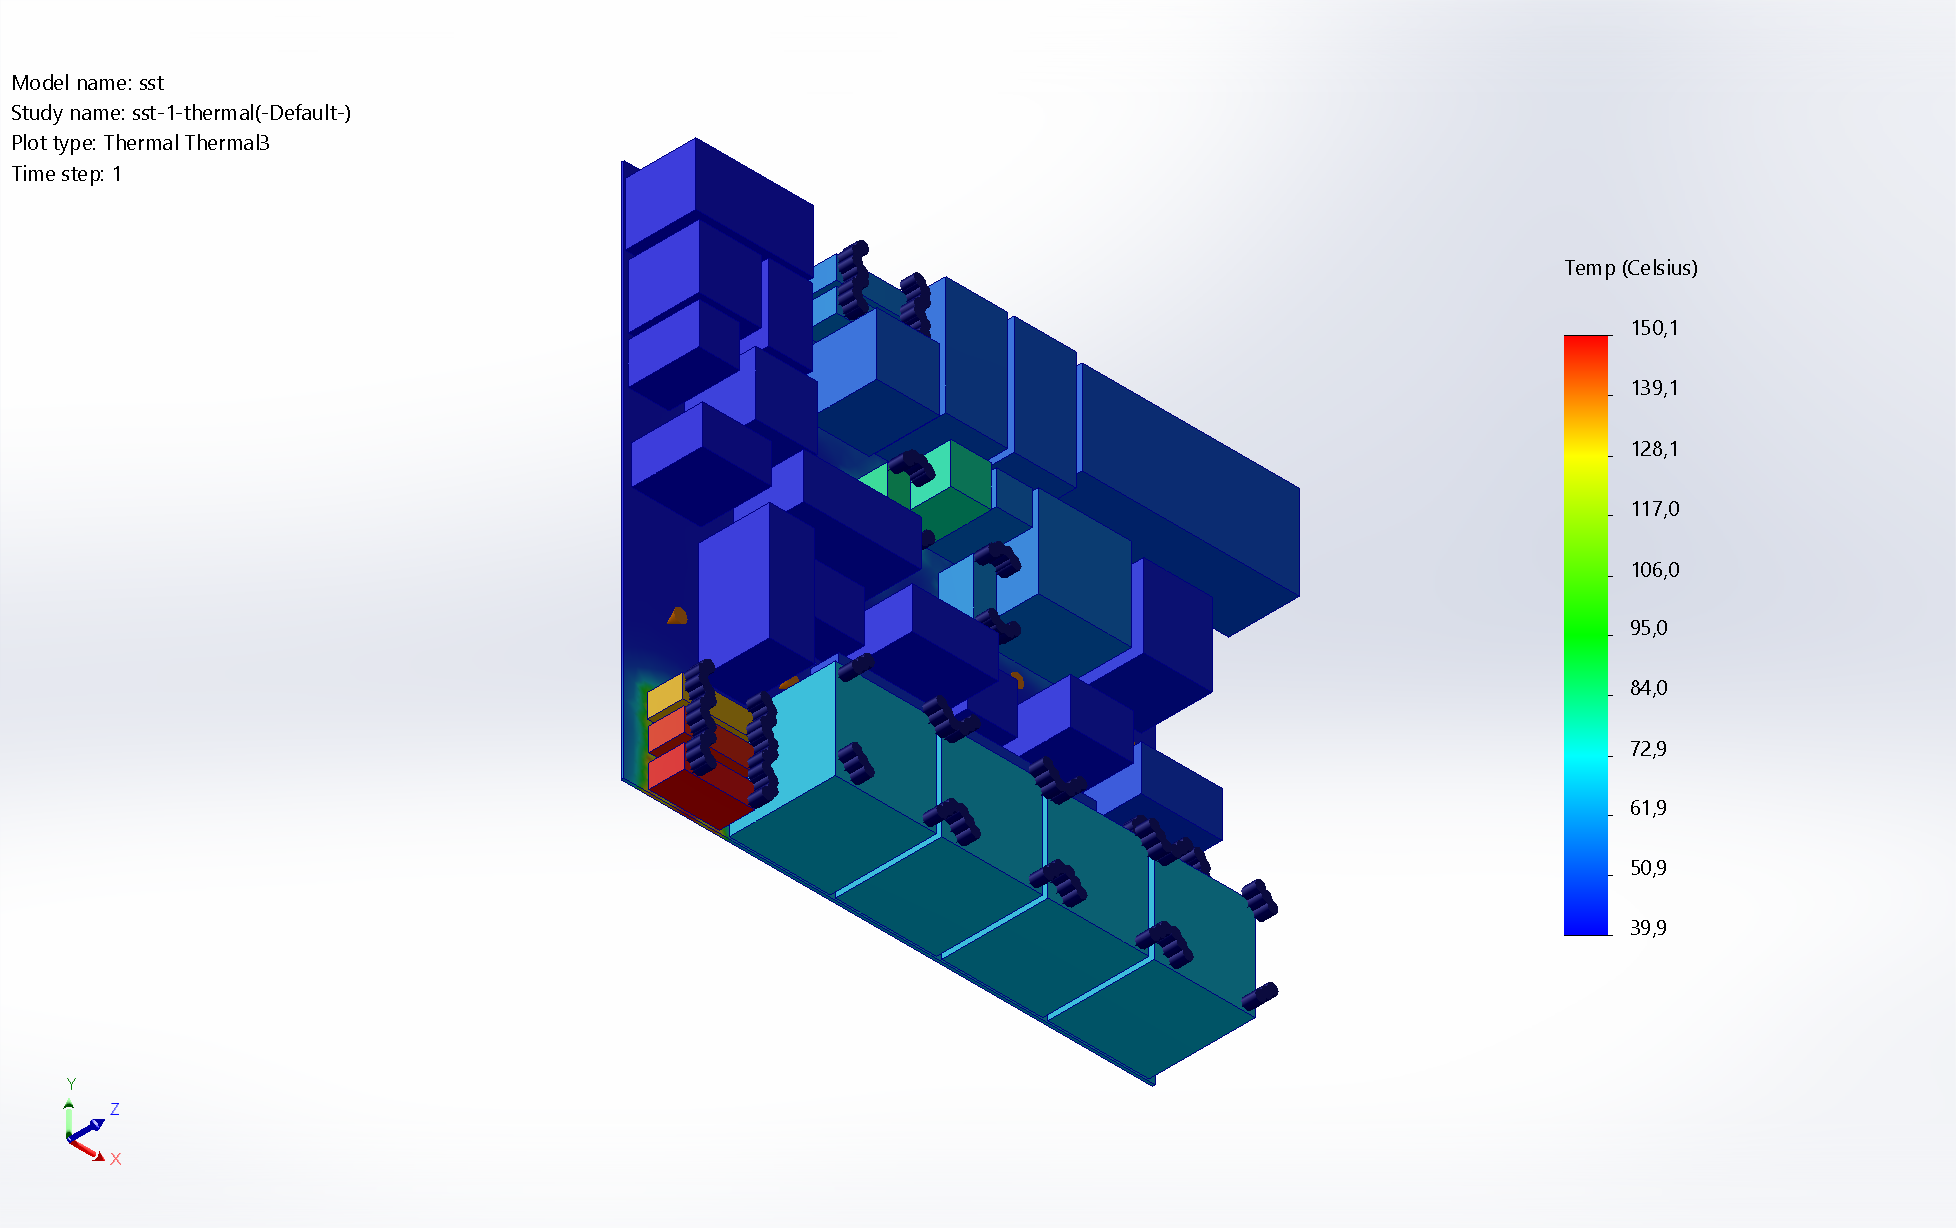
\includegraphics[scale=0.3]{../img/sst-1/thermal/top_view.png}
  \caption{Результаты теплового анализа в \textit{SOLIDWORKS Simulation}
    для первого варианта компоновки}
\end{figure}

Результаты теплового анализа для второго варианта компоновки ПП в
\textit{SOLIDWORKS Simulation} представлены на рисунке 15.

\begin{figure}[h]
  \centering
  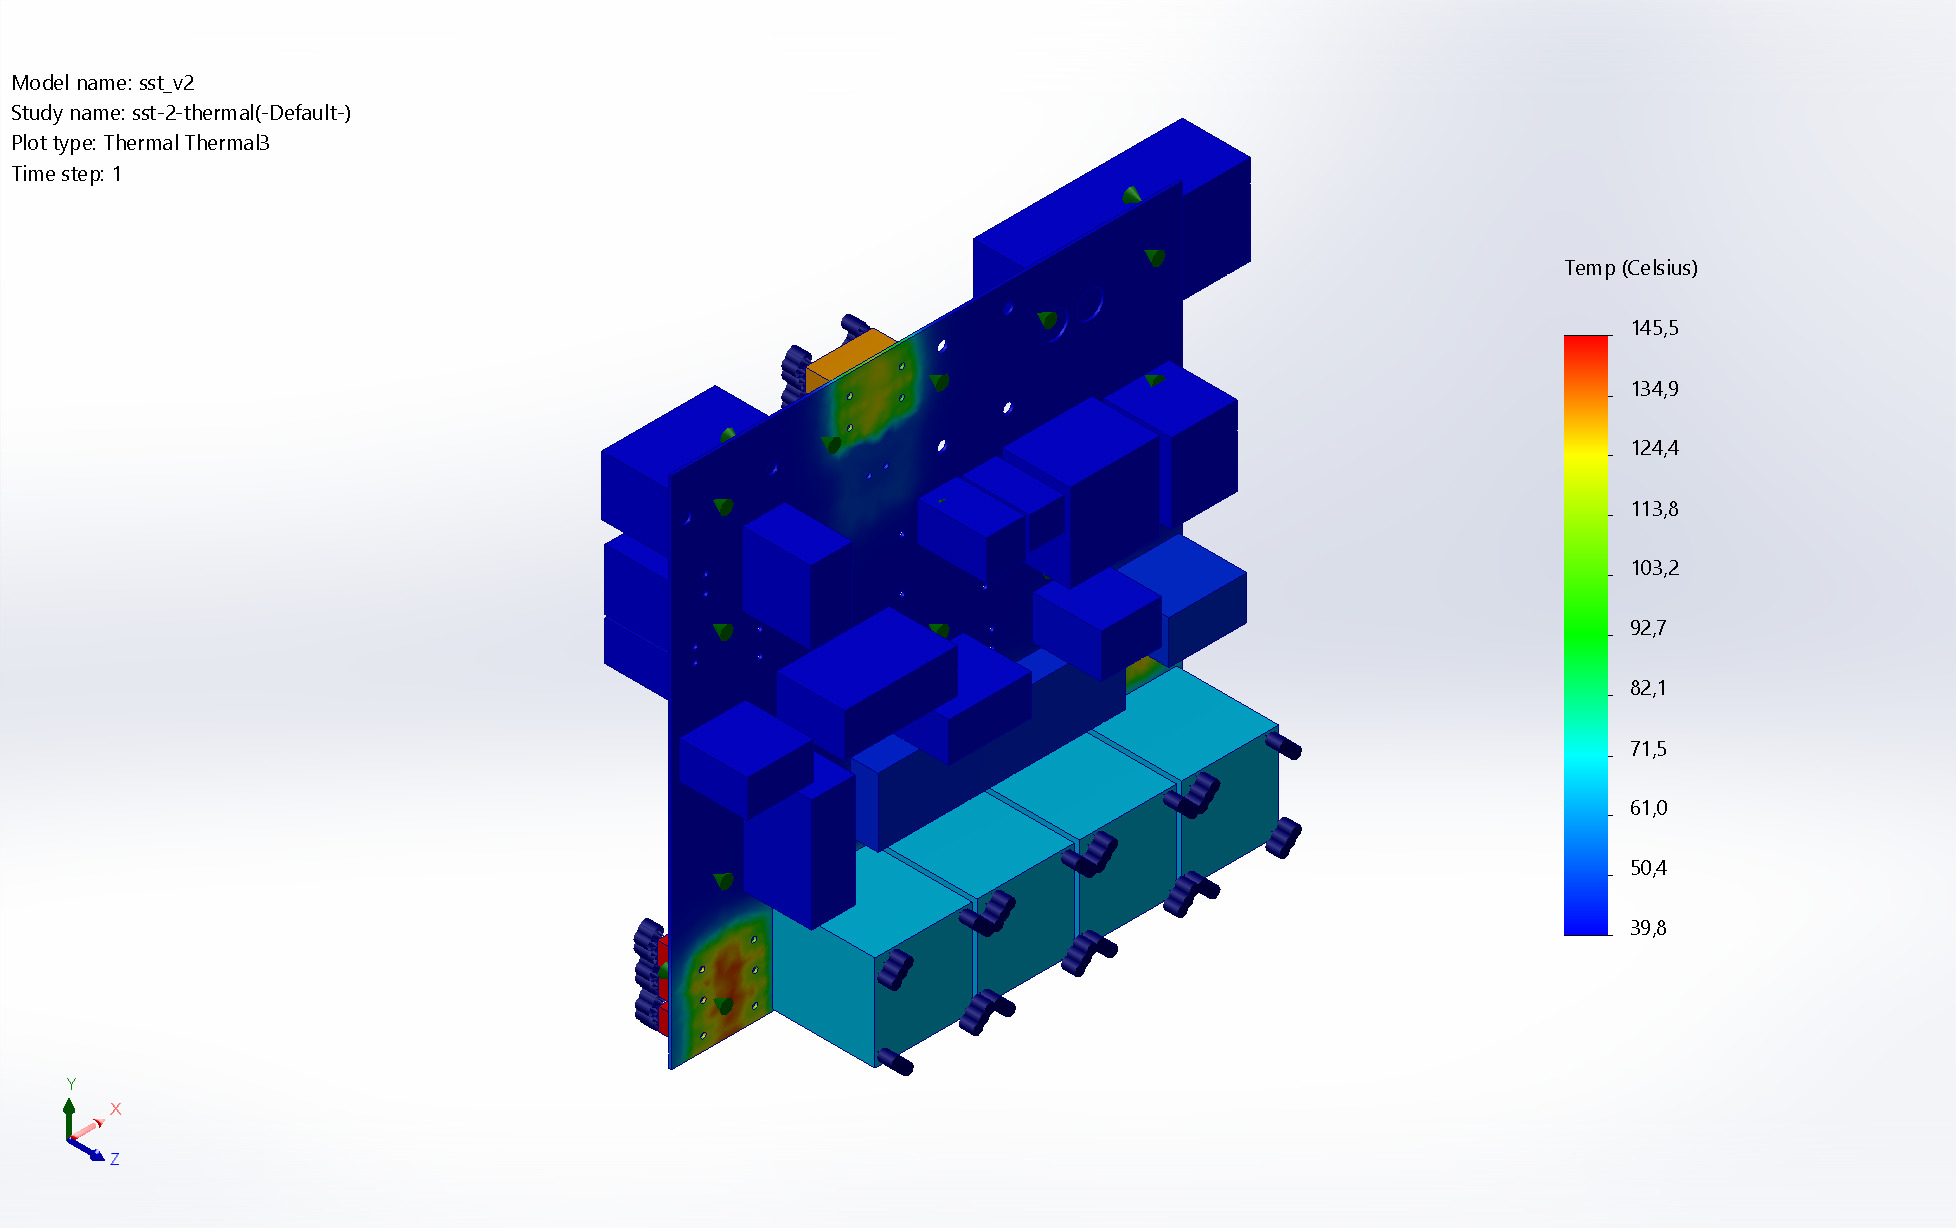
\includegraphics[scale=0.3]{../img/sst-2/thermal/sst_v2-sst-2-thermal-Thermal-Thermal3.jpg}
  \caption{Результаты теплового аналиаза в \textit{SOLIDWORKS Simulation}
    для второго варианта компновки}
\end{figure}

Результаты теплового анализа для третьего варианта компоновки ПП в
\textit{SOLIDWORKS Simulation} представлены на рисунке 16.
\begin{figure}[h]
  \centering
  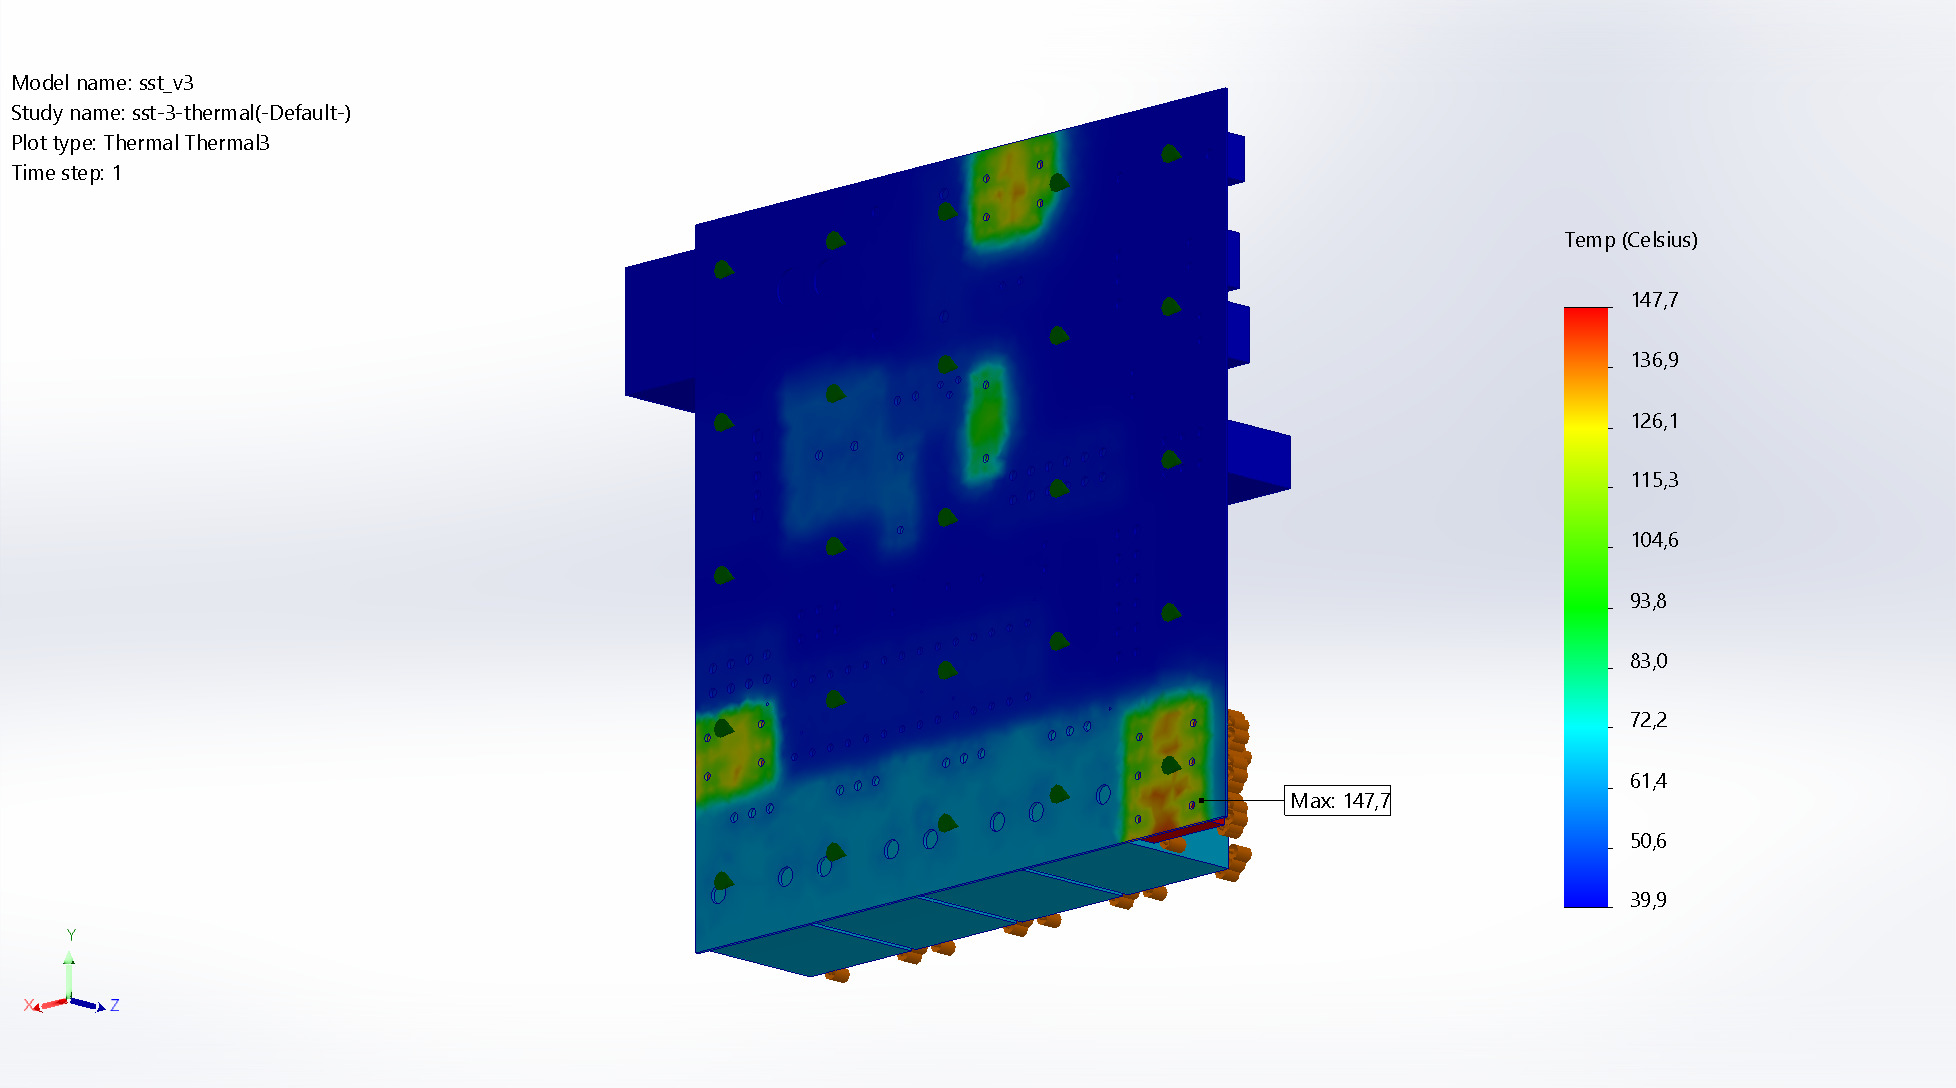
\includegraphics[scale=0.3]{../img/sst-3/thermal/sst_v3-sst-3-thermal-Thermal-Thermal3.jpg}
  \caption{Результаты теплового аналиаза в \textit{SOLIDWORKS Simulation}
    для второго варианта компновки}
\end{figure}

Результаты тепловго анализа для первого варианта компоновки ПП в
\textit{COMSOL Multiphysics} представлены на рисунке 17.
\begin{figure}[h]
  \centering
  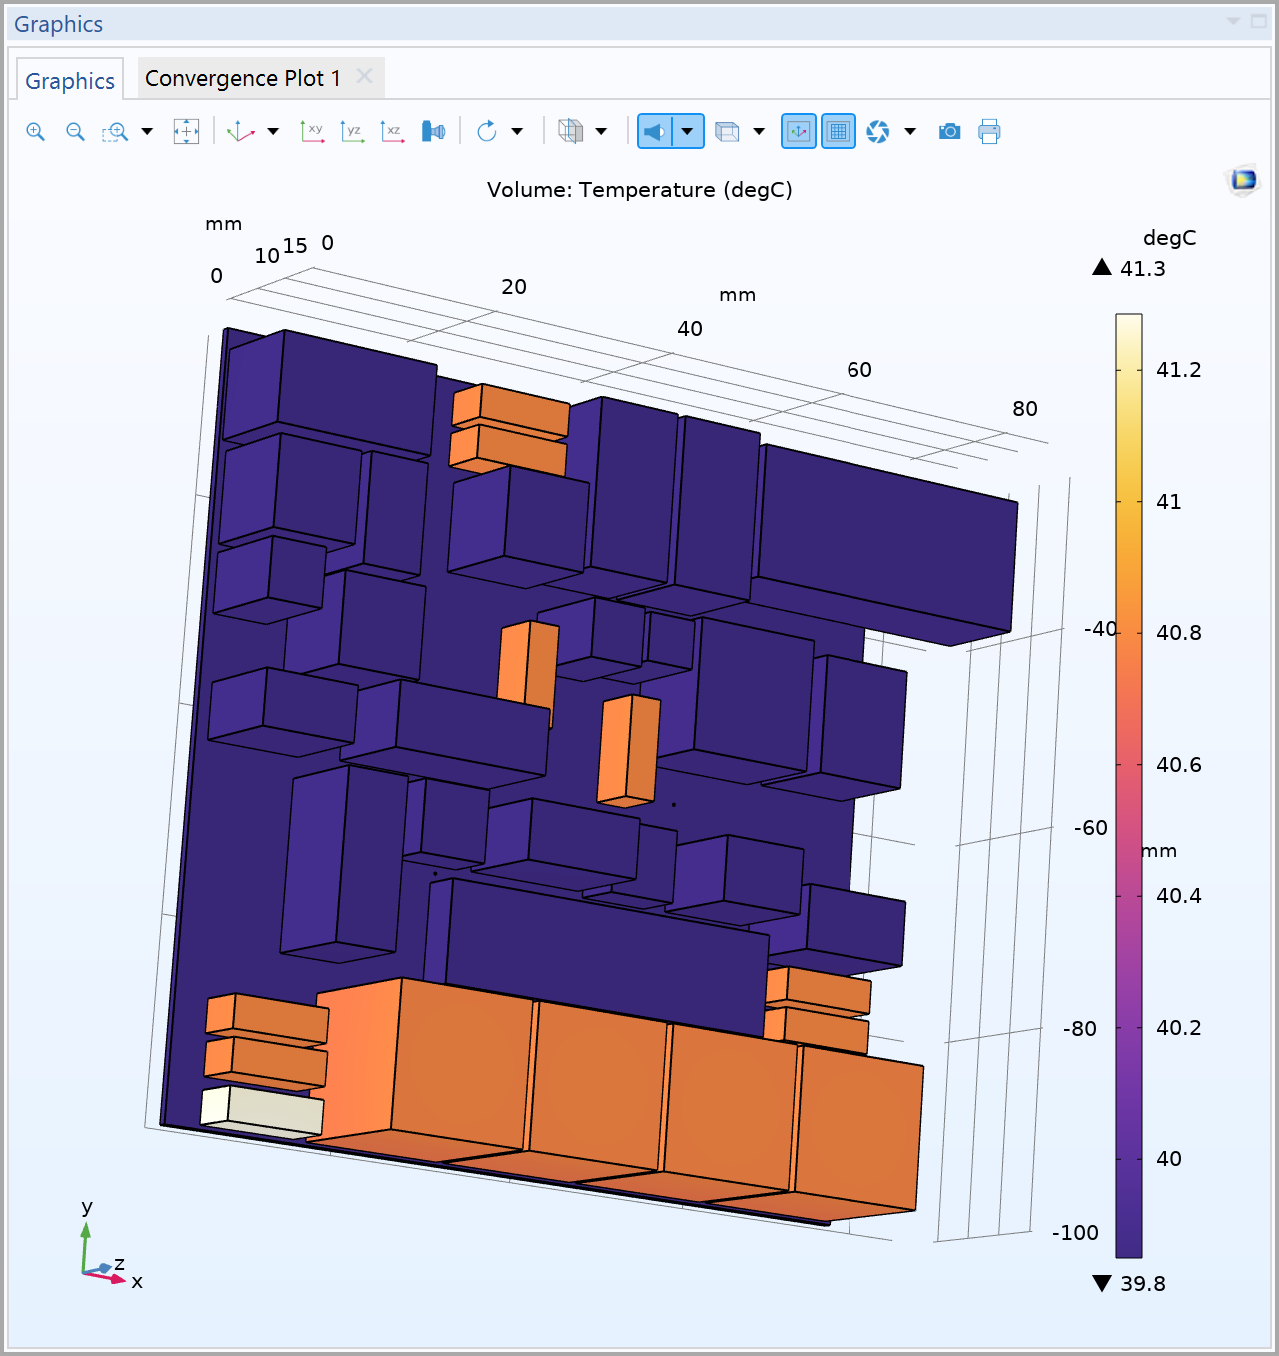
\includegraphics[scale=0.5]{../img/scrot/Screenshot-2024-05-16-022638.png}
  \caption{Результаты теплового анализа в \textit{COMSOL Multhiphysics}
    для первого варианта компоновки}
\end{figure}

Результаты теплвого анализа для второго варианта компоновки ПП в
\textit{COMSOL Multiphysics} представлены на рисунке 18.

\begin{figure}[h]
  \centering
  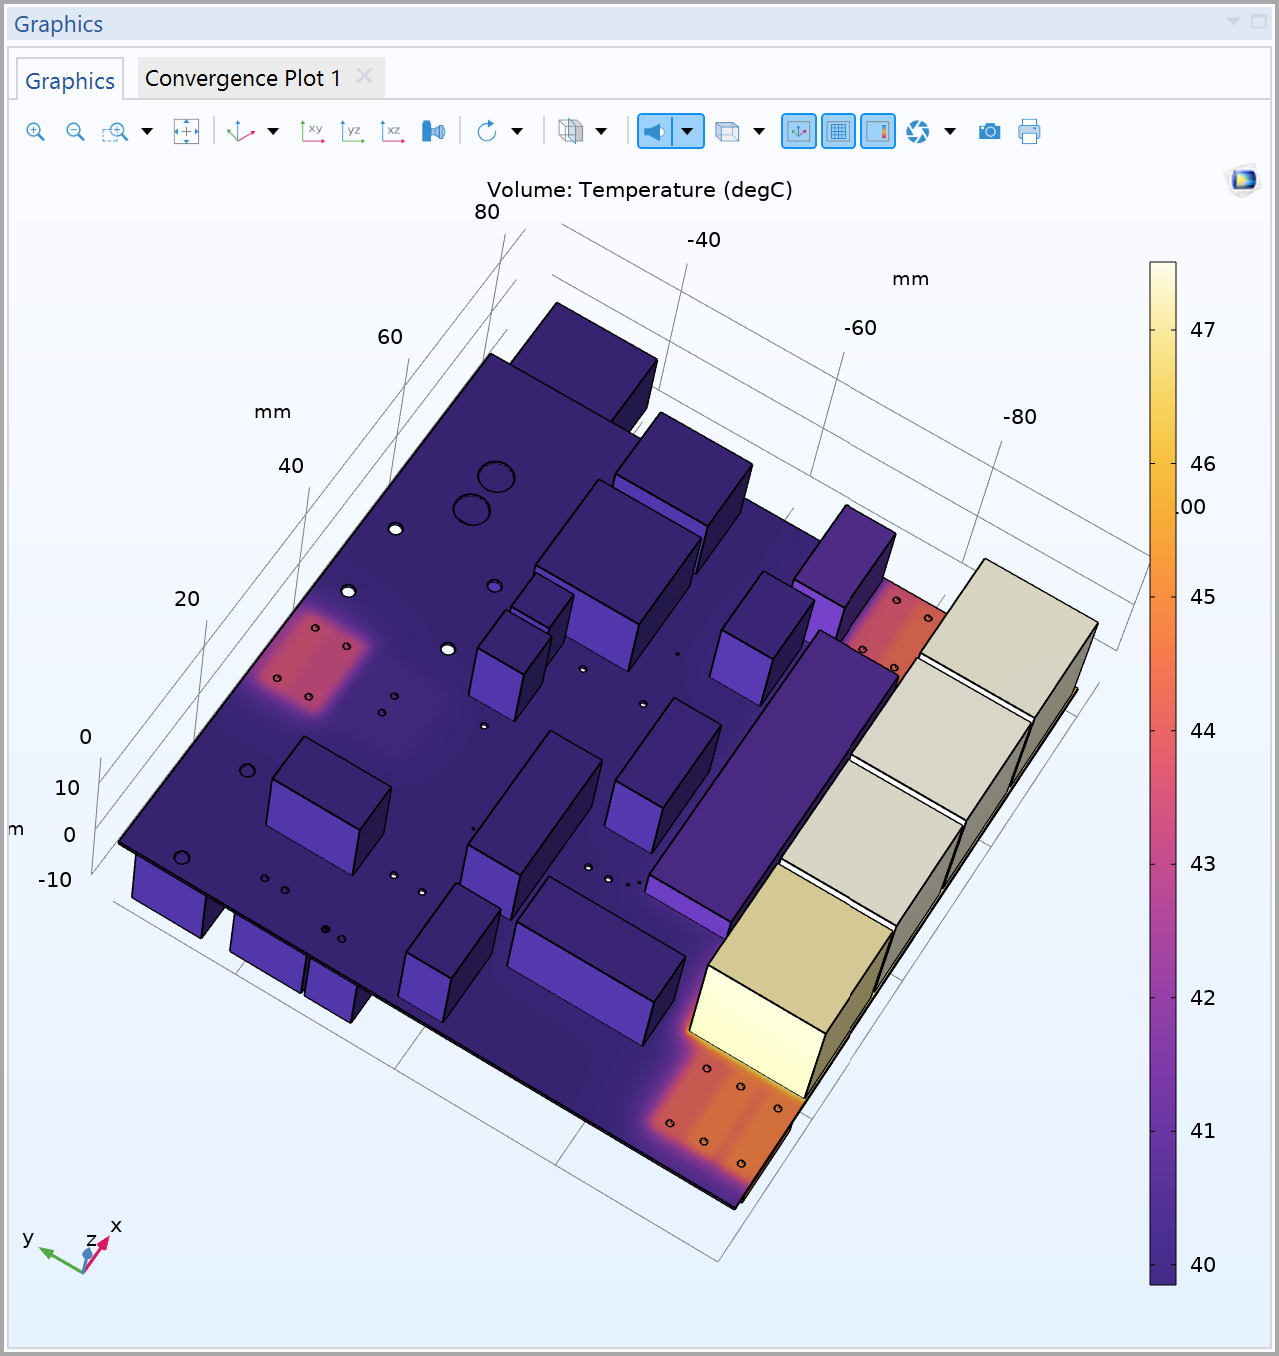
\includegraphics[scale=0.5]{../img/scrot/Screenshot-2024-05-16-023133.png}
  \caption{Результаты теплвого анализа в \textit{COMSOL Multiphysics}
  для второго варианта компоновки}

\end{figure}

Результаты тепловго анализа для третьего варианта комопновки ПП в
\textit{COMSOL Multiphysics} представлены на рисунке 19.
\begin{figure}[H]
  \centering
  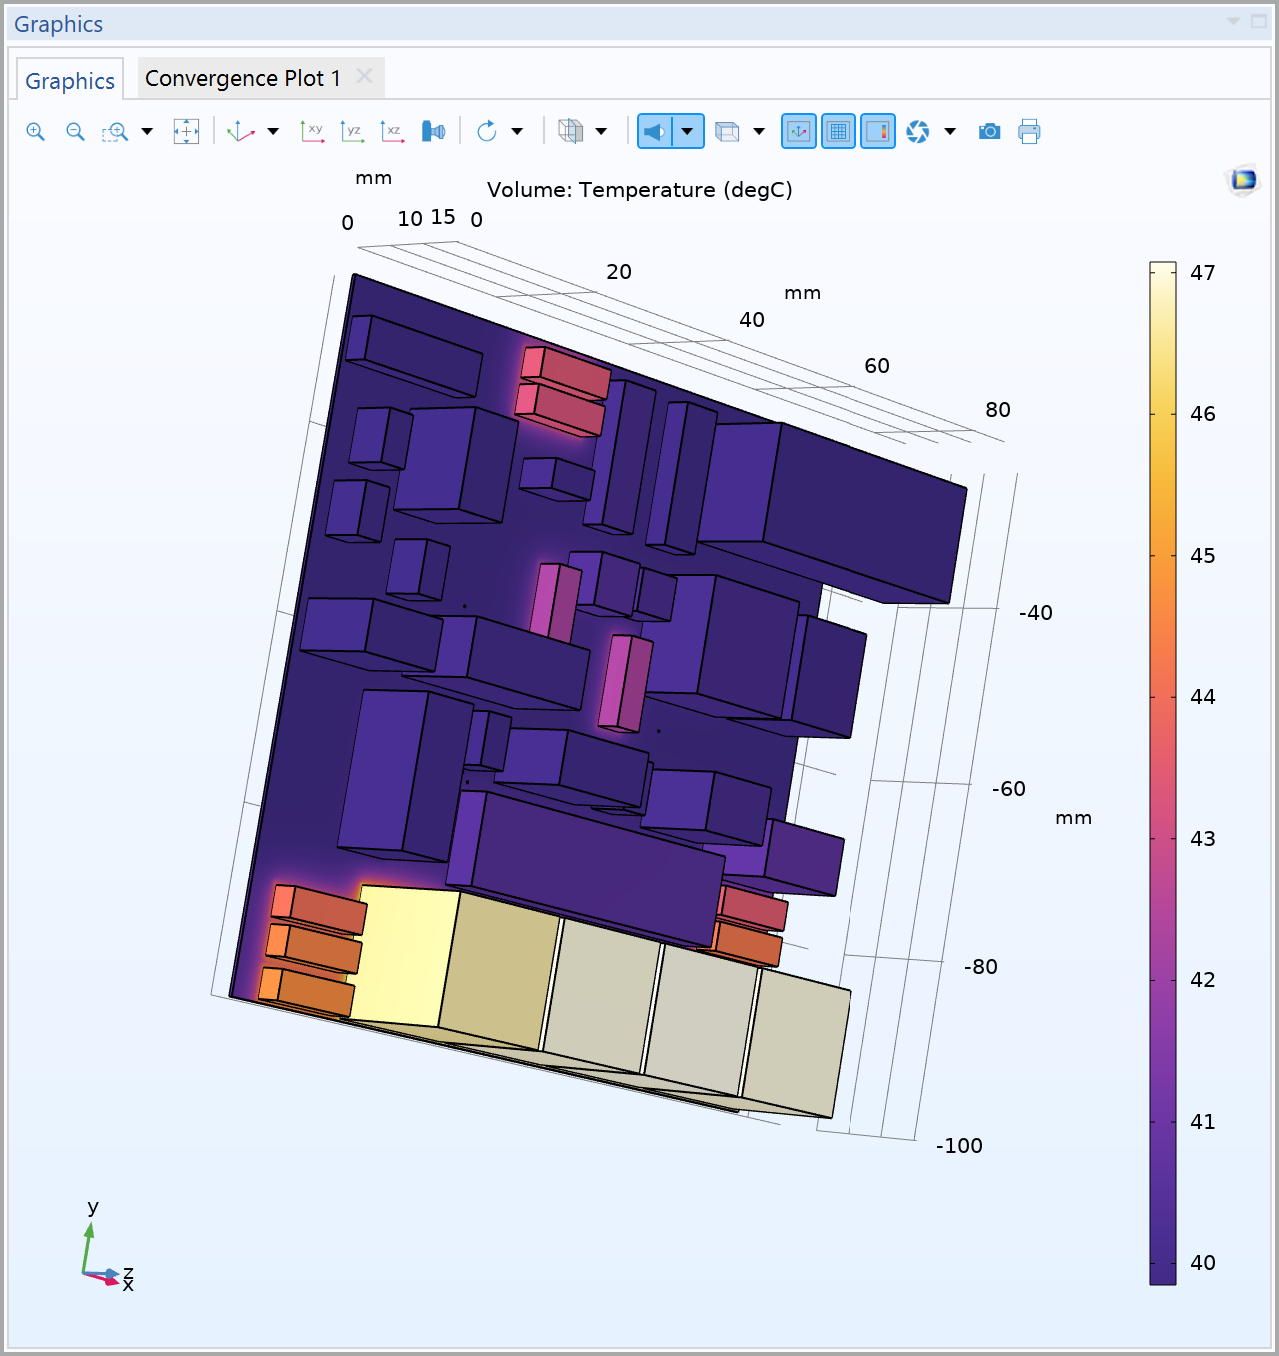
\includegraphics[scale=0.5]{../img/scrot/Screenshot-2024-05-16-024105.png}
  \caption{Результаты теплвого анализа в \textit{COMSOL Multiphysics}
  для третьего варианта компоновки}

\end{figure}





\newpage
\section{Анализ полученных результатов моделирования}
\subsection{Обработка, анализ и интепретация данных проведенного моделирования механических процессов}

\begin{table}[h]
  \centering
  \caption{Результаты частотного анализа в \textit{SolidWorks}}
\begin{tabular}{|c|c|}
\hline
  Вариант компоновки ПП & Значение собственной частоты \\
  1 & 10,1Гц \\
  2 & 7,3 Гц \\
  3 & 7,9 Гц \\
\hline
\end{tabular}
\end{table}

Самое большое значение частоты у печатной платы выполненненой в первой компоновке. Однако можно заметить, что во всех трёх случаях частота досточно мала. 10 Гц это 10 колебаний платы в секунду, что несоотвевует уровню требуему данной печатной плате.

Однако можно считать, что в значительной степени такой результат вышел потому, что плата крепилась только за одну поверхность и была очень тонкой, так как такой вышла модель в результате экспорта.

\begin{table}[h]
  \centering
  \caption{Результаты частотного анализа в \textit{COMSOL Multiphysics}}
\begin{tabular}{|c|c|}
\hline
  Вариант компоновки ПП & Значение собственной частоты \\
  1 & 0.1 Гц \\
  2 & 13509 Гц \\
  3 & 14 Гц \\
\hline
\end{tabular}
\end{table}

Результаты анализа в \textit{COMSOL Multiphysics} так разнятся, что сделать какой-либо вывод, а не исключить данные из анализа сложно.
Но судя по всем именно значение 13509 Гц ближе всего к тому значению, которое должно было получиться при анализе печатной платы в независомости от компоновки.


\subsection{Обработка, анализ и интепретация данных проведенного моделирования телповых процессов}

\begin{table}[H]
  \centering
  \caption{Результаты теплового анализа в \textit{SolidWorks}}
\begin{tabular}{|c|c|}
\hline
  Вариант компоновки ПП & Максимальное начение температуры в Цельсиях \\
  1 &  150 \\
  2 &  145 \\
  3 &  143 \\
\hline
\end{tabular}
\end{table}

Самое большое значение температуры у печатной платы в первой компановке.
По видимому оба решения с разнесеним компонентов по разные стороны платы
и заменой тепловыделяющих компонентов на меньшие по размеру выглядят приемлимыми для обеспечения теплового режима ПП.

Но только теплового режима  печатной платы.

\begin{table}[H]
  \centering
  \caption{Результаты теплового анализа в \textit{COMSOL Multiphysics}}
\begin{tabular}{|c|c|}
\hline
  Вариант компоновки ПП & Значение максимальной температуры в Цельсиях \\
  1 & 41.3 \\
  2 & 47,5 \\
  3 & 47 \\
\hline
\end{tabular}
\end{table}

Моделирование в \textit{COMSOL Multiphysics} показало ровно противоположный результат. При этом в качестве геометрии была импортирована модель из \textit{SOLIDWORKS} с расширением \textit{.SLPDRT}

По видимому несовпадение результатов вызвано различным методом решения применямым в данных программах.

Однако я склонен больше доверять \textit{COMSOL}, как программер специально предназначенных для таких рассчетов.

По полученным результатам и графикам можно сделать вывод,
что при проектировании печатной платы, точнее при, так называемой разводке, решение о том как расставлять компоненты можно принимать
не только основываясь на том как близко должен быть элемент с точки зрения схемотехники, но также учитывать, что рассеивающие тепло в значительной степени компоненты будут нагреваться до больших температур в тех случаях, когда будут расставлены рядом.

\newpage

\begin{center}
\textbf{Заключение}
\end{center}

В результате выполнения курсового проекта проведен общетехнический
анализ проектируемого устройства, который включает: анализ исходных данных, описание принципа работы анализируемого устройства, анализ электрической принципиальной схемы устройства, определение параметров воздействующих дестабилизирующих факторов и протекающих физических процес-
лсов для последующего моделирования.

Проведено моделирование физических процессов, воздействующих на
устройство, а именно: обоснование выбора прикладного программного обеспечения для моделирования физических процессов, разработан план моделирования физических процессов, разработана методика построения трехмерной модели исследуемого устройства, проведено моделирование механических
процессов, протекающих в электронном модуле и устройстве в целом, и проведено моделирование тепловых процессов, протекающих в электронном модуле и устройстве в целом.
Основываясь на вышеперечисленном, был проведен анализ полученных
результатов, а также дана краткая оценка.

Таким образом была предпринята попытка реализовать все поставленные цели и задачи на курсовой проект. Однако с уверенностью можно заключить, что эта попытка не была удачной. Большую роль сыграли проблемы с экспортом модели трехмерной модели, случившиеся в результате перехода на другую систему автоматизированного проектирования печатной платы.

Остается только сделать выводы и не допускать ошибок, подобных допущенным при выполнении данного курсового проекта.
  \newpage



% \bibligoraphystyle{5sem}
% \renewcommand{\bibsection}{{Cписок использованных источников}}
\renewcommand{\refname}{\textbf{Cписок использованных источников}}
\DeclareFieldFormat{url}{Режим доступа\addcolon\space\url{#1}}
\DeclareFieldFormat{title}{{#1}}
\DeclareFieldFormat{labelnumberwidth}{[{#1}]\adddot  }
\printbibliography

\newpage
\begin{center}
\textbf{Приложение А}\\
\textbf{Обязательное}\\
\textbf{Параметры компонентов}
\end{center}

Техническое описание ПП:
\begin{enumerate}[label={\arabic*.}]
\item Соотношение сторон 1:1.
\item Габариты ПП 75 на 75 мм.
\item Толщина ПП 0,8 мм.
\end{enumerate}

Данные необходимые для тепловго анализа:
\begin{enumerate}[label={\arabic*.}]
\item Температура окружающей среды 315 К.
\item Коэффициент конвекции — 25 Вт/К * м².
\end{enumerate}

\newpage


\begin{center}
\textbf{Приложение Б}\\
\textbf{Обязательное}\\
\textbf{Отчет о проверке на заимствования в системе «Антиплагиат»}

\begin{figure}[H]
  \centering
  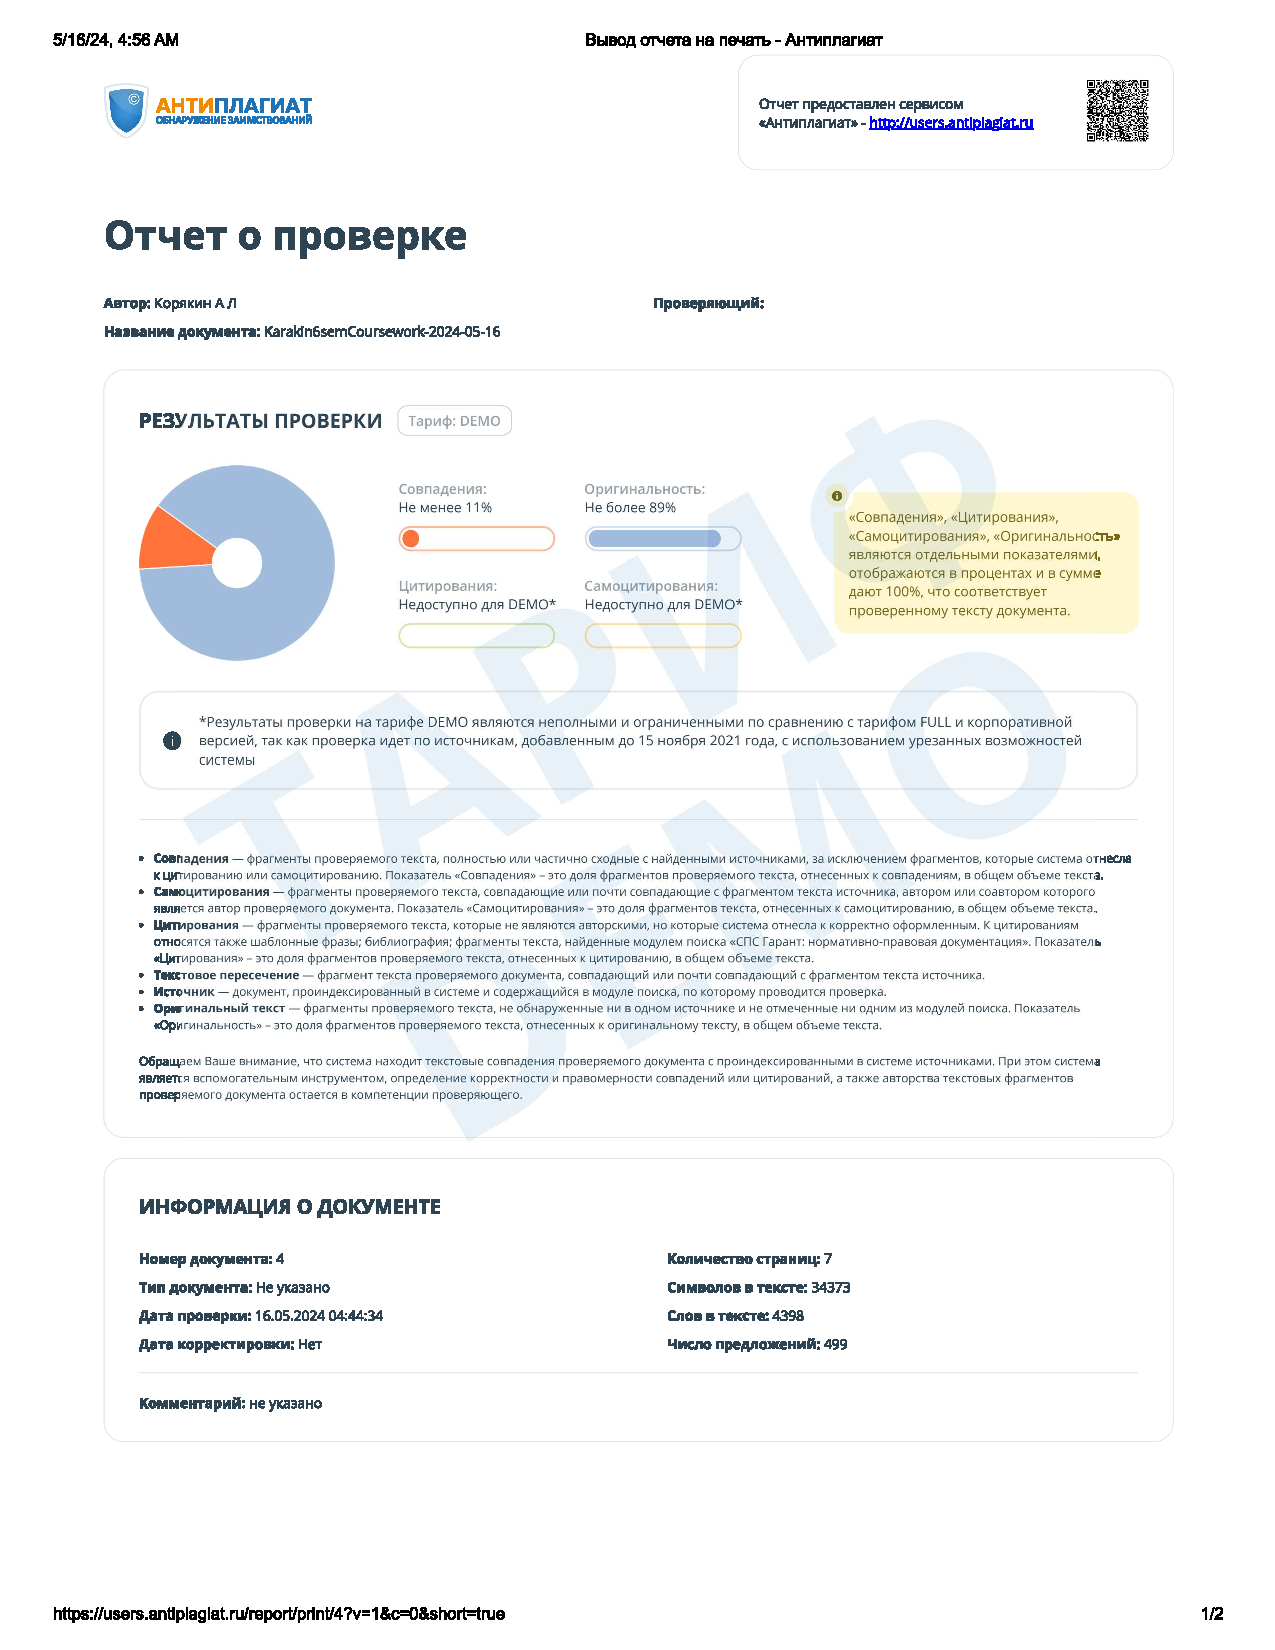
\includegraphics[scale=0.7]{../img/antiplagiat.pdf}
  \caption{Результат проверки на заимстования в системе «Антиплагиат»}
\end{figure}
\end{center}

\end{document}
